\chapter{Introducción}
\label{chap:introduccion} 
Este Trabajo Fin de Grado se enmarca en el ámbito educativo, en concreto en la \textit{Gamificación} de una plataforma web de robótica educativa. Según avanza la ciencia y la tecnología la sociedad ha cambiado y las formas de enseñar también. Este proyecto tiene como objetivo crear nuevos juegos y ejercicios que permitan enseñar a programar a los más jóvenes de una forma más divertida para fomentar el aprendizaje y la motivación, así como mejorar sus habilidades. Este proyecto engloba numerosas tecnologías web y herramientas que han servido para crear nuevos ejercicios para la plataforma de robótica educativa \textit{Kibotics} \cite{intro}.

En este primer capítulo se hace una breve introducción de la Robótica y de las tecnologías web, conceptos clave para ponernos en contexto y enfatizar en el tema principal de este trabajo: la \textit{``Gamificación''}.


%%%%%%%%%%%%%%%%%%%%%%%%%%%%%%%%%%%%%%%%%%%%%%%%%%%%%%%%%%%%%%%%%%%%%%%%%%%%%%%%%%%%%%%%%%%%%%%%%%%%%%%%%%%%%%%%
\section{Robótica}\label{motivacion}
La Robótica es una rama de la ingeniería que combina las matemáticas, la electrónica, la mecánica, la informática y la física. Gracias a la unión de estas ramas de conocimiento se han podido desarrollar sistemas electromecánicos llamados robots. 

Un robot es una máquina autónoma o semi-autónoma que es capaz de percibir su entorno, realizar cálculos para tomar decisiones, actuar en el mundo real de acuerdo con esas decisiones y comunicarse con otras máquinas o con humanos. Un robot se compone principalmente de 4 elementos:
\begin{itemize}
  \item Sensores: para recibir información de su entorno (láser, lídar, ultrasonidos (Figura 1.1), infrarrojos, cámaras, radio frecuencia, sensores térmicos...). 
   
  \item Actuadores:  permiten la locomoción del robot por su entorno y manipulación de objetos (motores eléctricos, de combustión, amortiguadores, hélices, servomotores (Figura 1.3), patas, ruedas, cadenas...). 
  

  \item  Controladores: Procesador (Figura 1.2) y algoritmos, para el cálculo y toma de decisiones. 
 
  \item Leds, pantallas (Figura 1.4), antenas, altavoces...: para comunicarse con otros robots o con humanos.
\end{itemize}
\begin{figure}[H] 
  \label{ fig7} 
  \begin{minipage}[b]{0.5\linewidth}
    \centering
    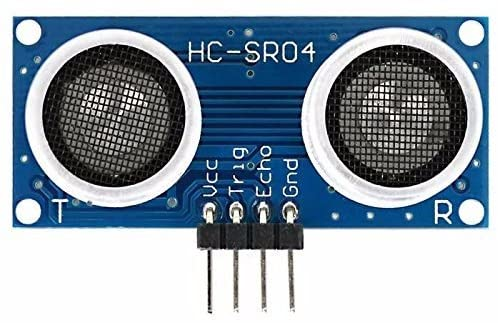
\includegraphics[width=.65\linewidth]{chapters/images/us.jpg} 
    \caption{Sensor ultrasonidos} 
  \end{minipage}%%
  \begin{minipage}[b]{0.5\linewidth}
    \centering
    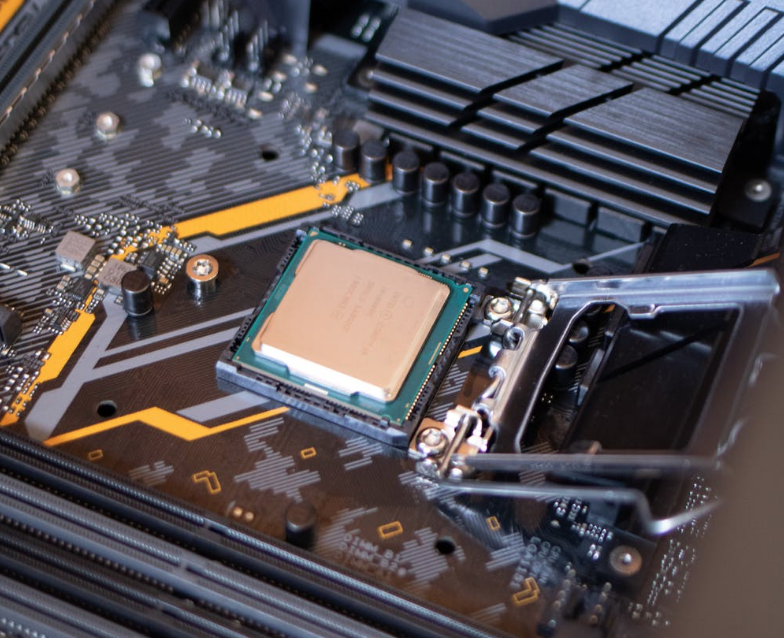
\includegraphics[width=.65\linewidth]{chapters/images/procesador.png} 
    \caption{Procesador} 
  \end{minipage} 
  \begin{minipage}[b]{0.5\linewidth}
    \centering
    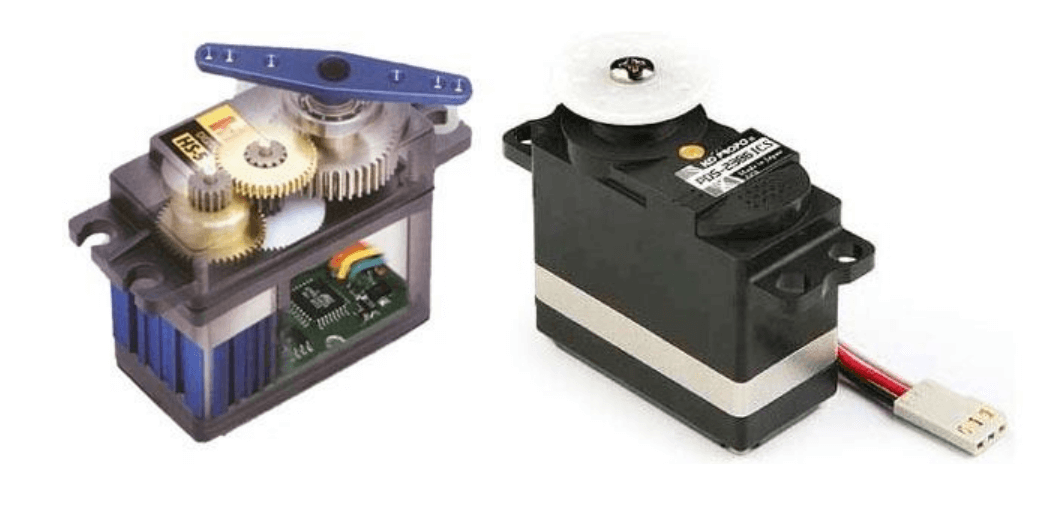
\includegraphics[width=.65\linewidth]{chapters/images/motor.png} 
    \caption{Servomotores} 
  \end{minipage}%% 
  \begin{minipage}[b]{0.5\linewidth}
    \centering
    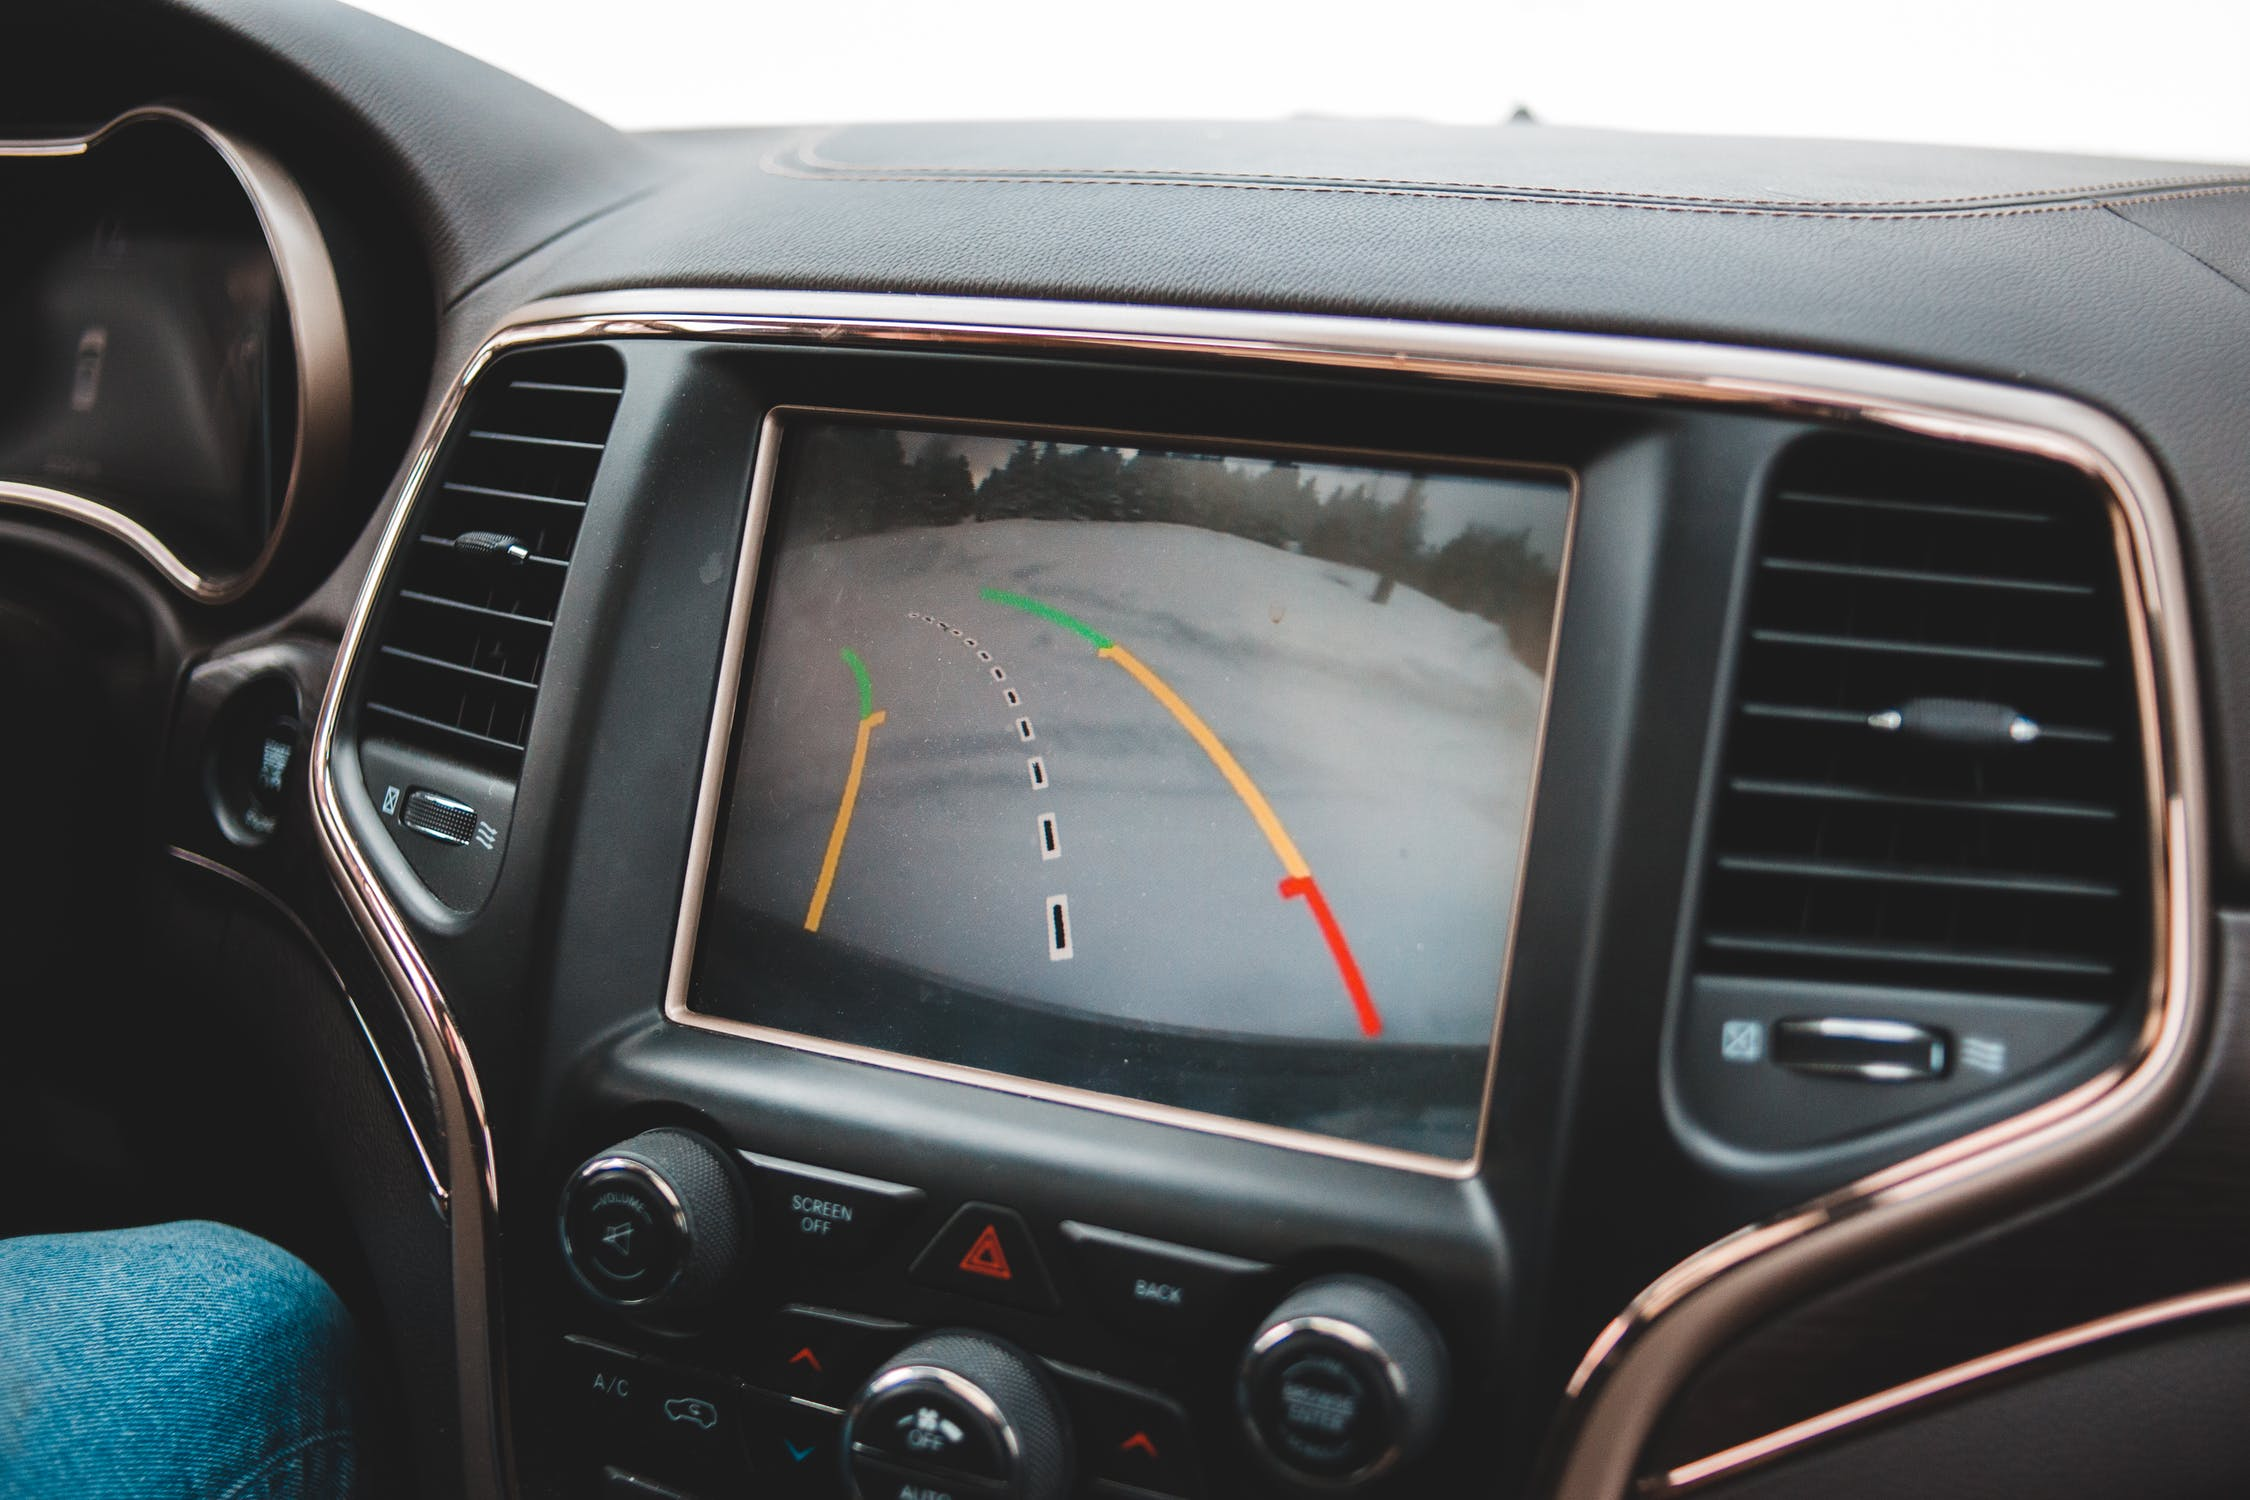
\includegraphics[width=.65\linewidth]{chapters/images/pantalla.jpeg} 
    \caption{Pantalla} 
  \end{minipage} 
\end{figure}

Los robots se clasifican según su entorno de aplicación en robots industriales y robots de servicio. También se pueden diferenciar según su forma en androides y zoomórficos, según su capacidad de movimiento en fijos o móviles, o según el medio en el que trabajan en terrestres, acuáticos o áereos. Estas son algunas de sus aplicaciones:
\begin{itemize}
    \item Robots industriales: brazos y pinzas robóticas para ensamblado de piezas, envasado de alimentos, industria automovilística y gestión de almacenes.
    \item Robots de servicio: destinados a limpieza del hogar, asistencia, coches autónomos, entrentenimiento, usos militares, limpieza de centrales nucleares, investigación en terrenos hostiles o fines médicos.
\end{itemize} 

 En la Figura 1.5 se muestran algunos ejemplos de robots que son de gran utilidad en la sociedad actual. 

\begin{figure}[H]
  \begin{subfigure}[b]{0.3\textwidth}
    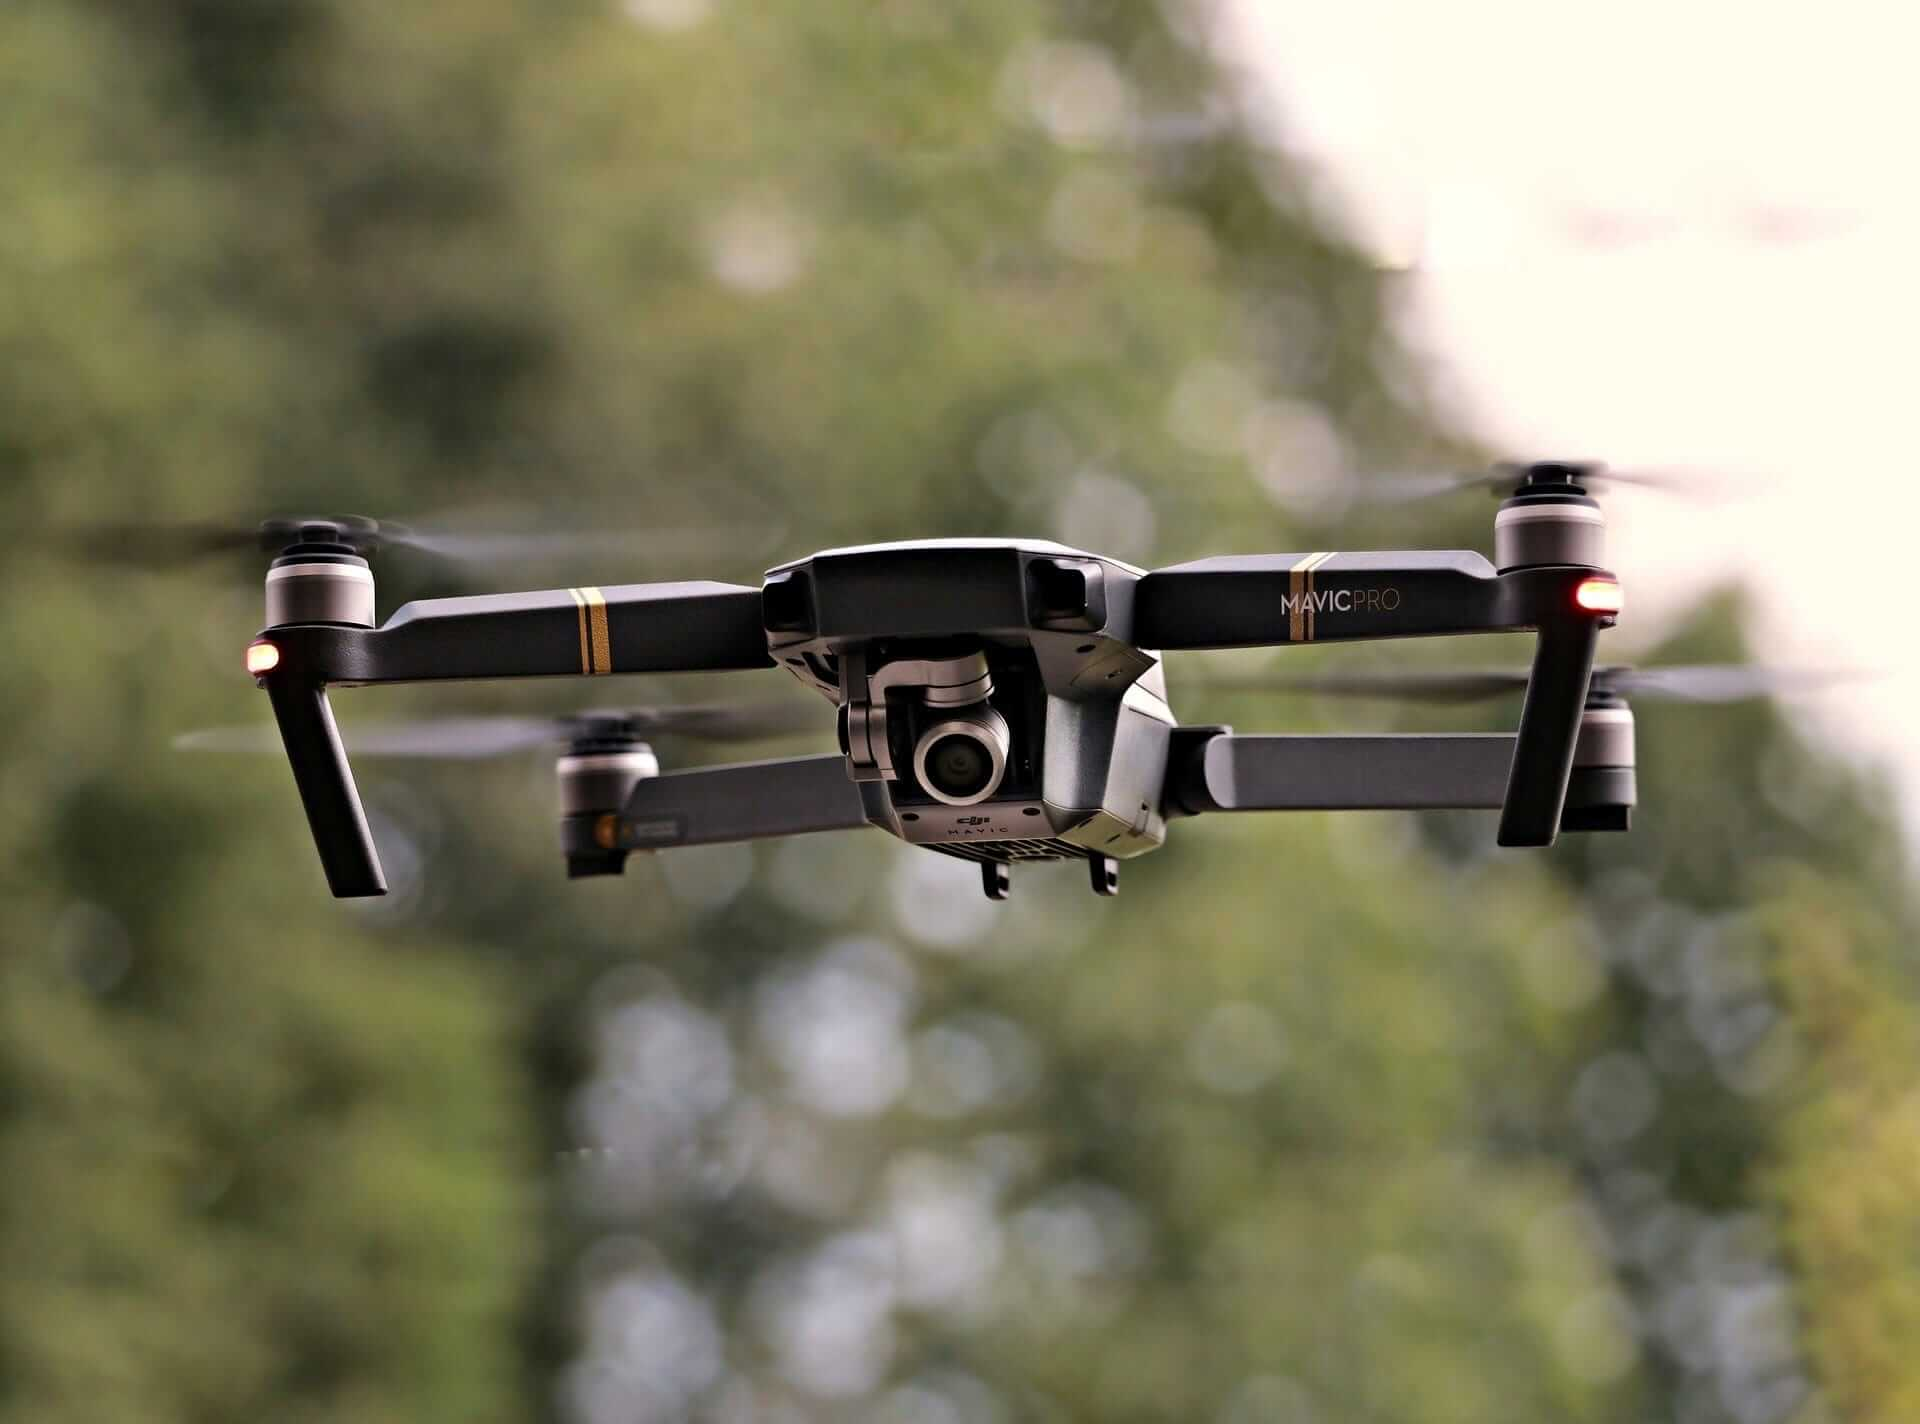
\includegraphics[width=\textwidth, height=\textwidth]{chapters/images/drone.jpeg}
    \caption{Dron}
    \label{fig:f1}
  \end{subfigure}
  \hfill
  \begin{subfigure}[b]{0.3\textwidth}
    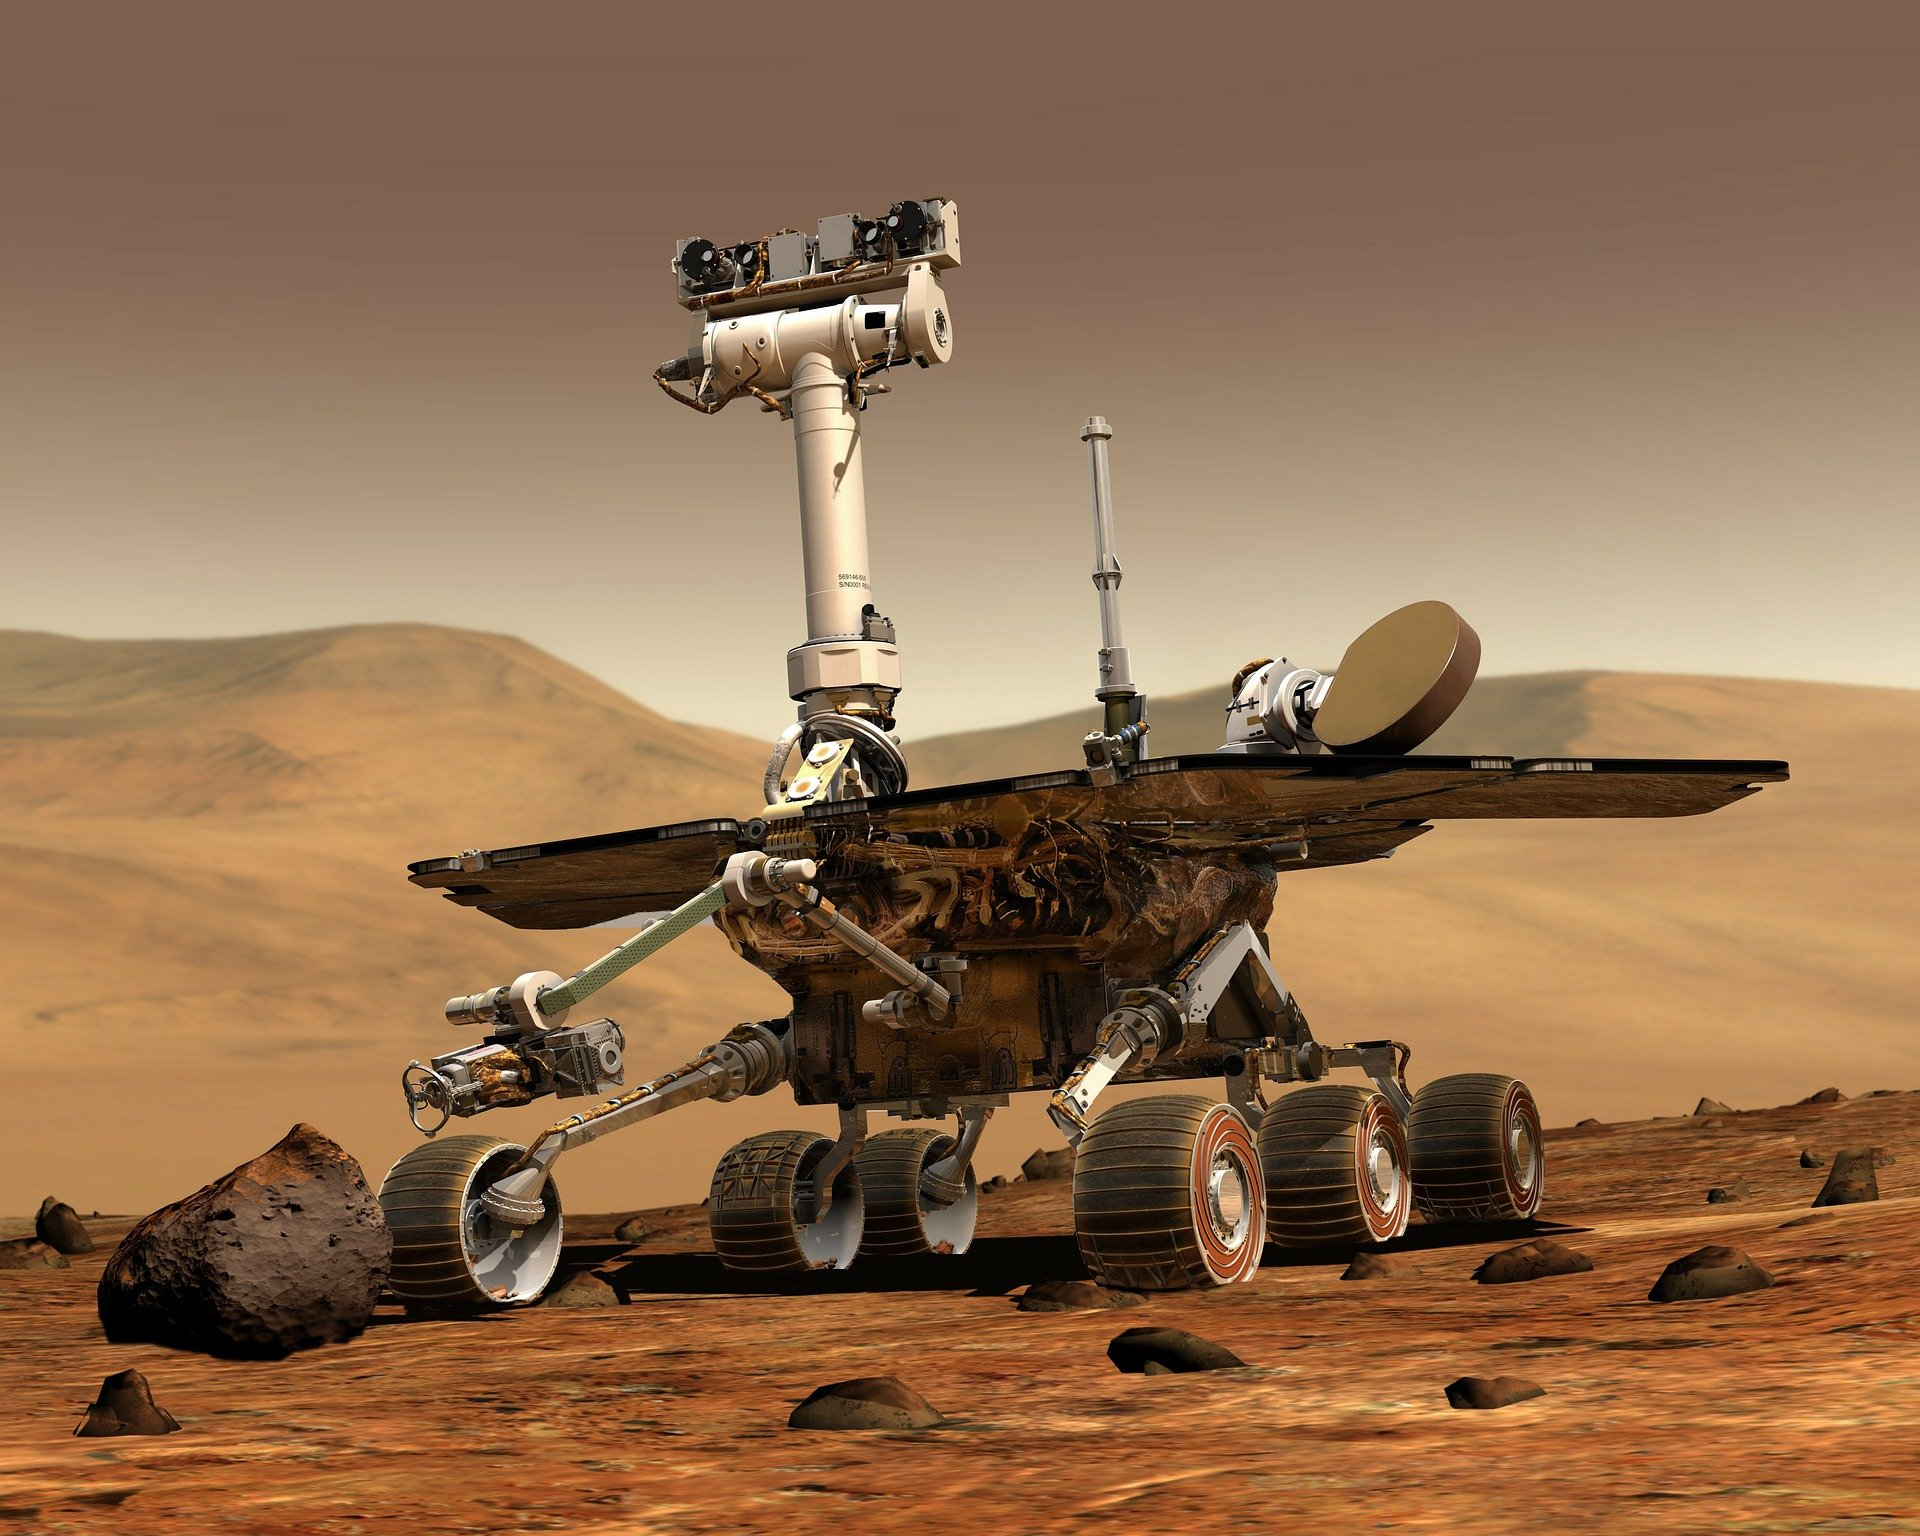
\includegraphics[width=\textwidth, height=\textwidth]{chapters/images/mars.jpg}
    \caption{Perseverance Mars}
    \label{fig:f2}
  \end{subfigure}
  \hfill
   \begin{subfigure}[b]{0.3\textwidth}
    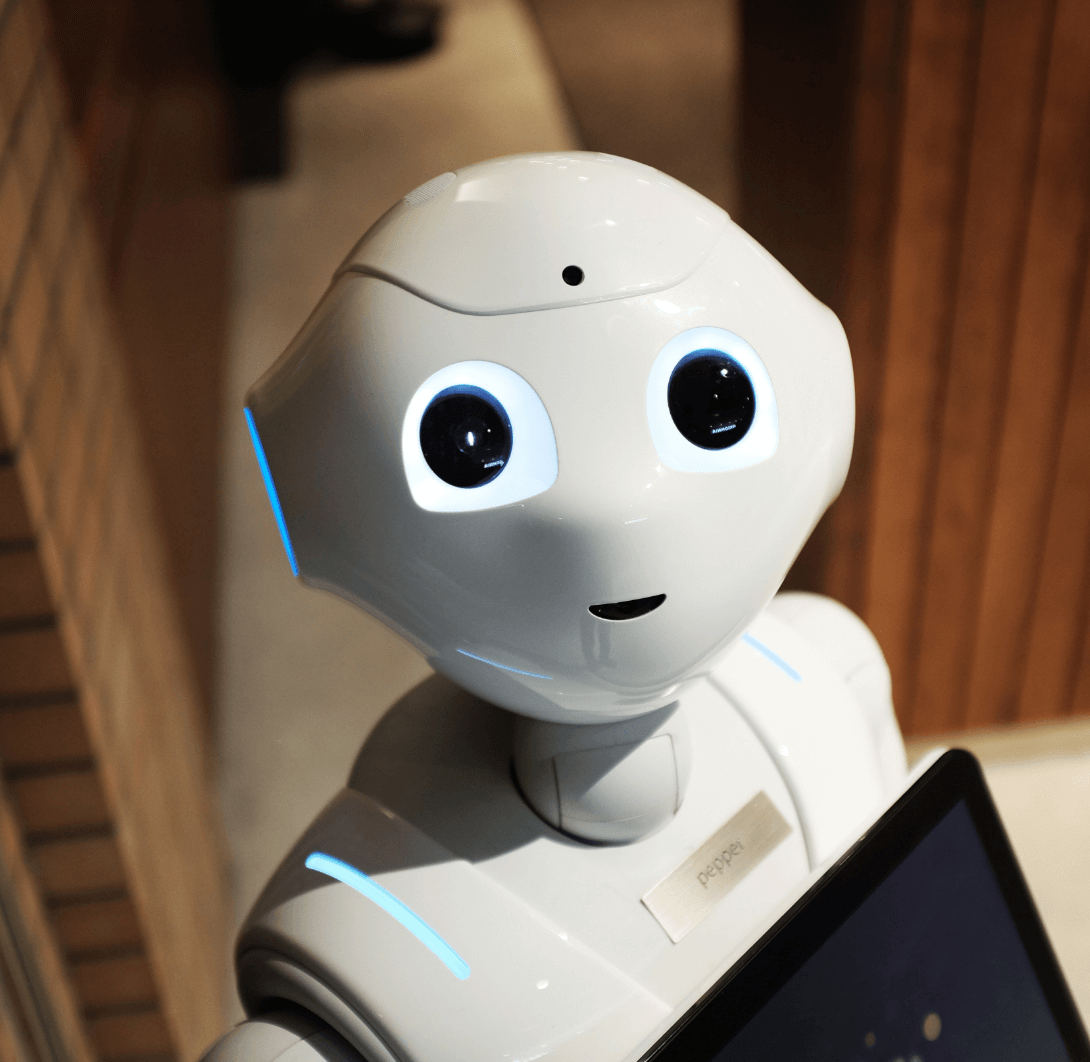
\includegraphics[width=\textwidth, height=\textwidth]{chapters/images/nao.png}
    \caption{Nao}
    \label{fig:f3}
  \end{subfigure}
  \hfill
   \begin{subfigure}[b]{0.3\textwidth}
    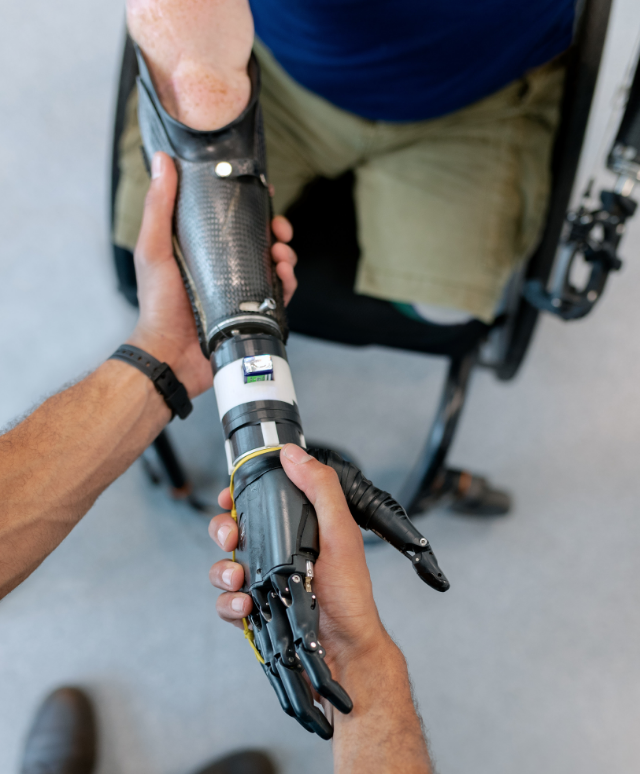
\includegraphics[width=\textwidth, height=\textwidth]{chapters/images/brazo.png}
    \caption{Brazo biónico}
    \label{fig:f4}
  \end{subfigure}
  \hfill
   \begin{subfigure}[b]{0.3\textwidth}
    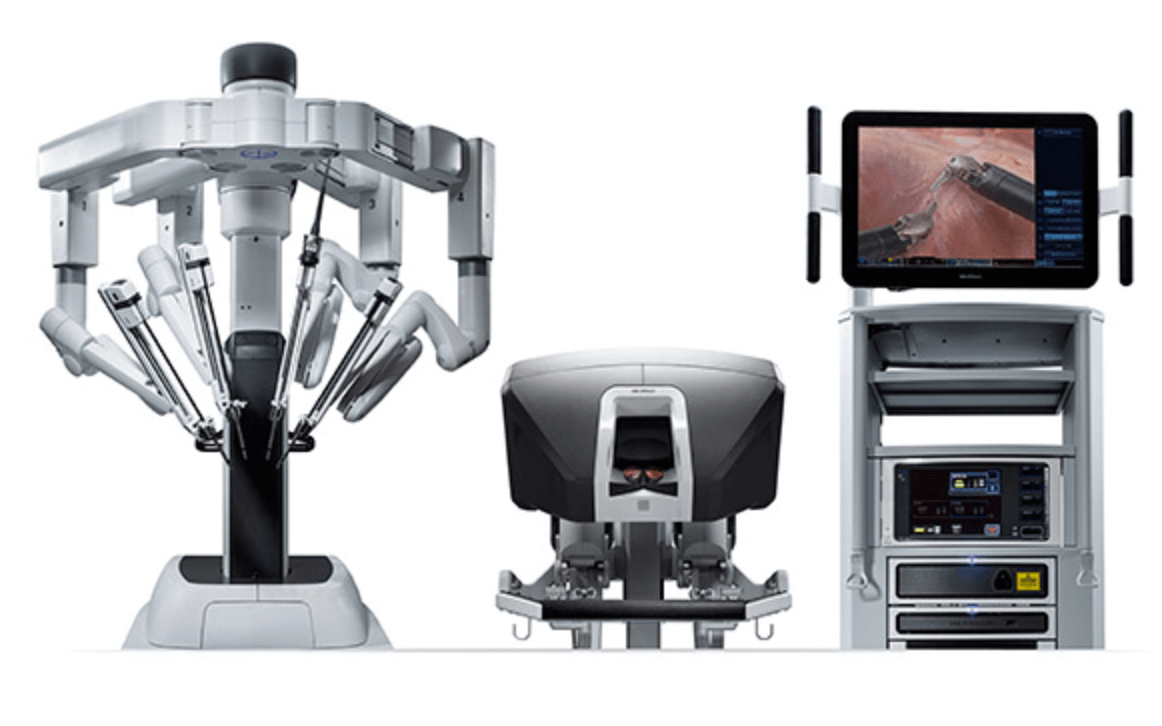
\includegraphics[width=\textwidth, height=\textwidth]{chapters/images/davinci.png}
    \caption{Da Vinci \cite{davinci} }
    \label{fig:f5}
  \end{subfigure}
  \hfill
   \begin{subfigure}[b]{0.3\textwidth}
    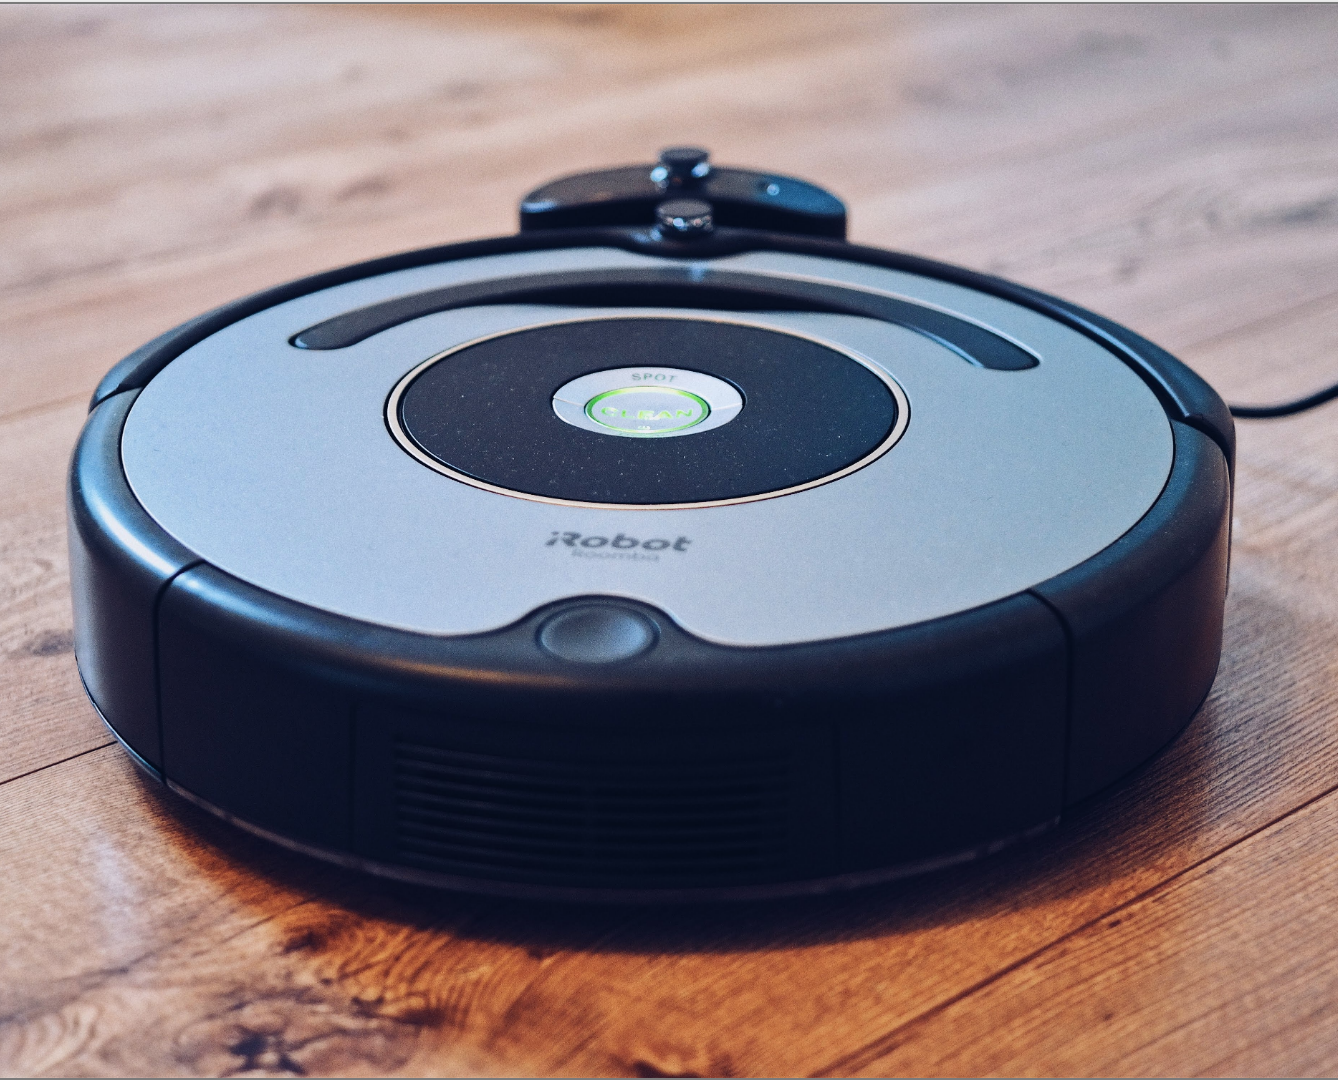
\includegraphics[width=\textwidth, height=\textwidth]{chapters/images/roomba.png}
    \caption{Roomba}
    \label{fig:f6}
  \end{subfigure}
  \caption{Ejemplos de Robots}
\end{figure}

La Figura 1.5(a) muestra un dron, estos pequeños vehículos no tripulados han sido toda una revolución en la grabación de eventos y películas. El entretenimiento no es su única aplicación, también se utilizan para la búsqueda de personas y vigilancia. 

El Perseverance Mars que vemos en la Figura 1.5(b) actualmente está en Marte haciendo investigaciones del terreno. Este robot busca signos de vida y guarda muestras para un futuro regreso a la Tierra.

Los robots de asistencia como el Nao, Figura 1.5 (c), son muy importantes para que los más pequeños y las personas mayores puedan socializar de una forma divertida y a su vez es una herramienta de apoyo en procesos de rehabilitación, post-operatorios y terapias ocupacionales.

Los brazos biónicos como el de la Figura 1.5(d) permiten recuperar las funciones y el tacto a amputados. El robot Da Vinci Figura 1.5(e) ayuda a los cirujanos a operar con mayor precisión y seguridad.  Estos robots han sido un gran avanze en el campo de la medicina.

El robot aspirador, uno del más conocido es \textit{Roomba}, Figura 1.5(f), es capaz de detectar obstáculos y residuos en el suelo. Esto nos ayuda a que la casa esté limpia y nos ahorra mucho tiempo.

Los robots que se han mencionado son solo algunos ejemplos. La robótica es una tecnología en auge. En los últimos años, con el avance de la tecnología, la realidad ha superado a la ficción, estamos rodeados de robots. Han salido de los laboratorios y han surgido miles de aplicaciones que nos hacen la vida un poco mejor.
\\
\\

Recientemente la robótica se está incorporando también a las aulas para que los más pequeños adquieran conocimientos y habilidades importantes para su futuro. En la siguiente Figura 1.6 se muestran unos ejemplos de robots diseñados para el ámbito educativo. \cite{roboticakids}

\begin{figure}[H]
    \centering
    \begin{subfigure}{.3\linewidth}
        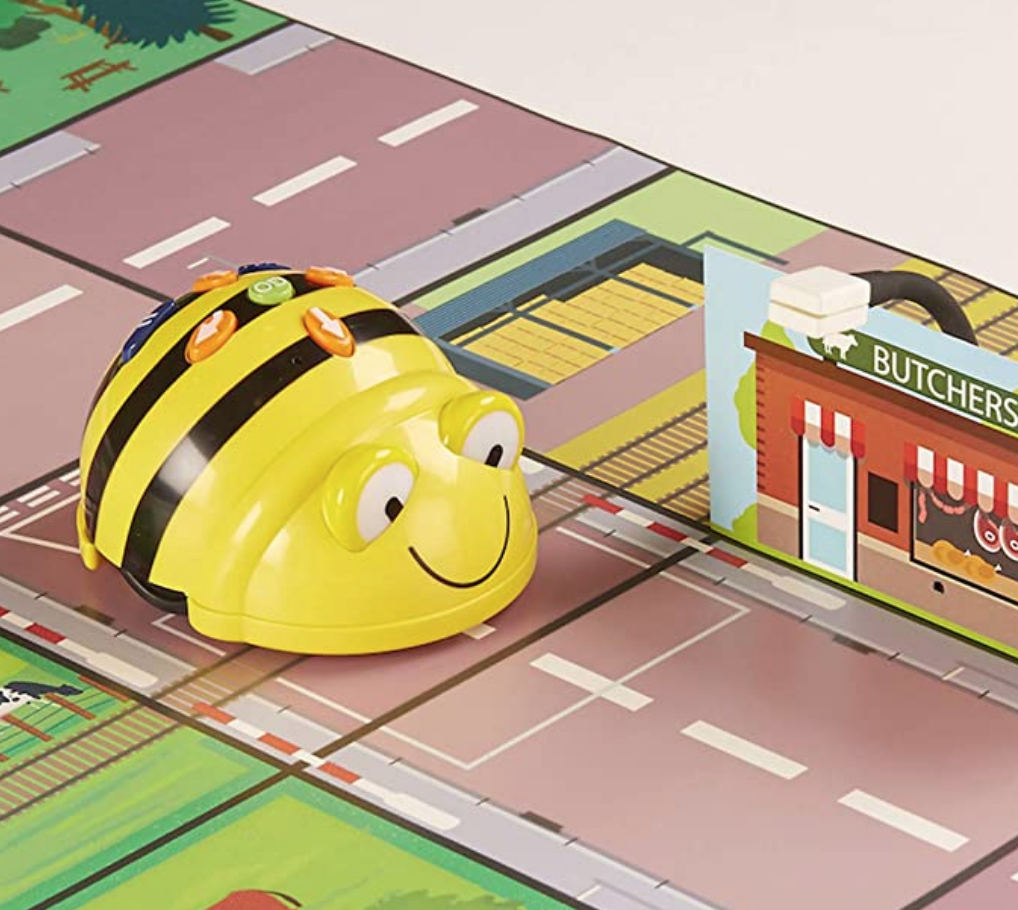
\includegraphics[width=1\textwidth]{chapters/images/beebot.png}
        \caption{Bee-bot}
    \end{subfigure}
    \hskip2em
    \begin{subfigure}{.3\linewidth}
    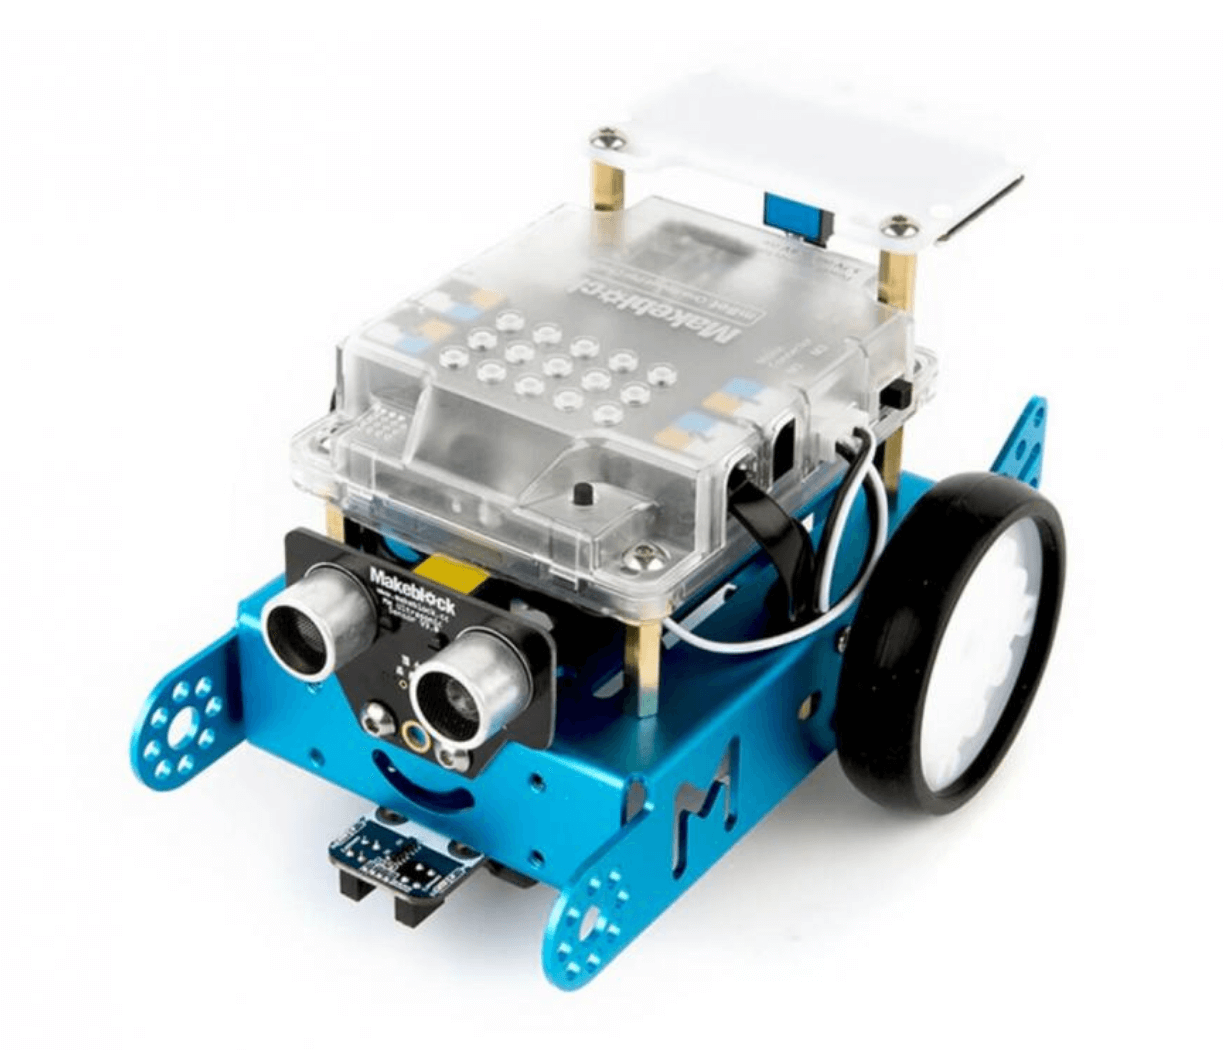
\includegraphics[width=1\textwidth]{chapters/images/mbot.png}
        \caption{Makeblock Mbot}
    \end{subfigure}
    \begin{subfigure}{.3\linewidth}
       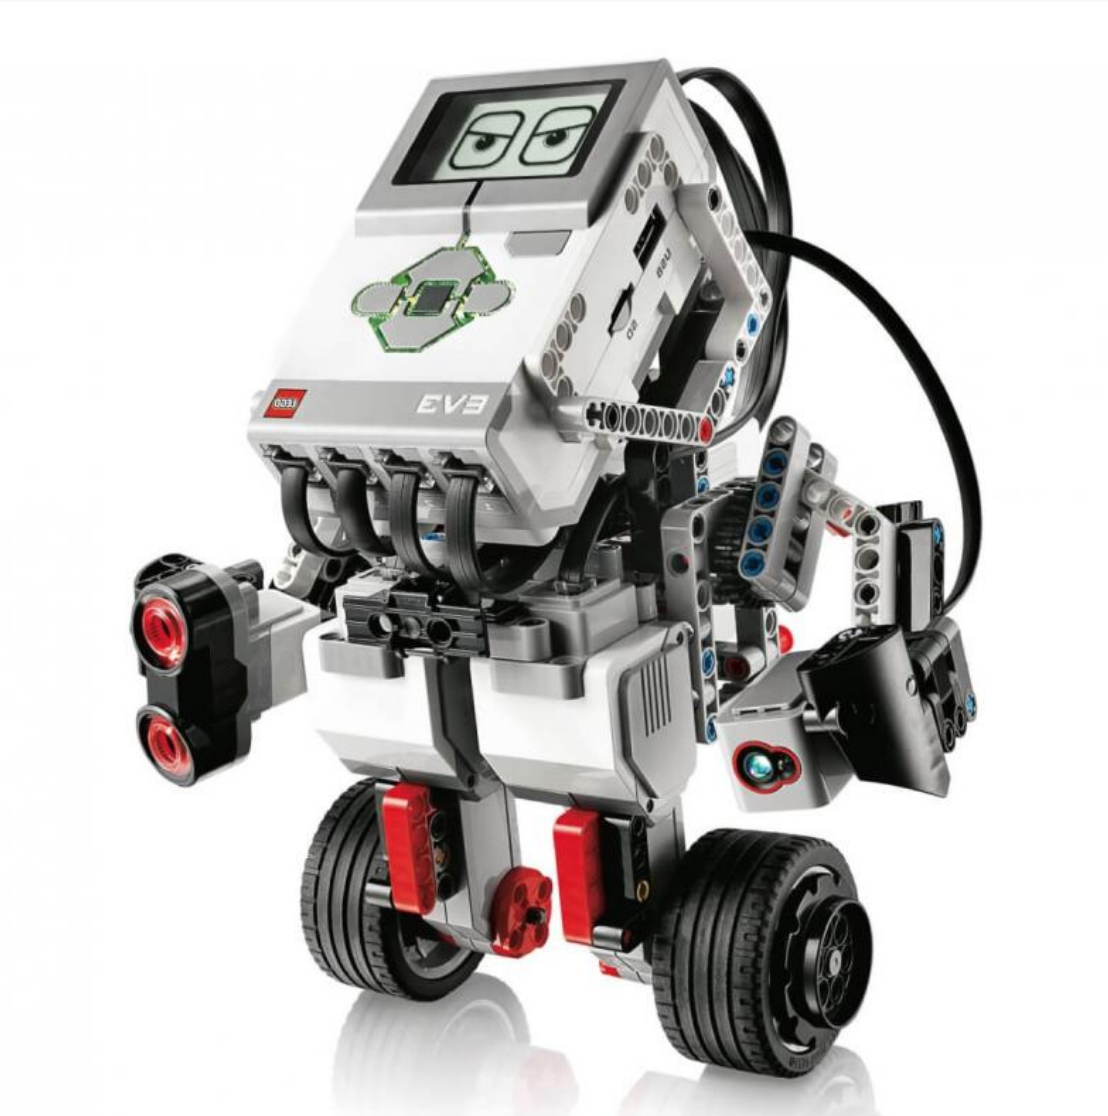
\includegraphics[width=1\textwidth]{chapters/images/lego.png}
        \caption{LEGO MINDSTORMS EV3}
    \end{subfigure}
    \caption{Ejemplos de Robots educativos}
\end{figure}


%%%%%%%%%%%%%%%%%%%%%%%%%
\newpage
\section{Tecnologías Web}
Las tecnologías web juegan un papel muy importante en el mundo moderno gracias a Internet. Esta plataforma WWW \footnote{World Wide Web}\cite{www}
ha ido evolucionando y ha posibilitado potentes aplicaciones con un modelo cliente/servidor. En la Figura 1.7 podemos ver algunos ejemplos de aplicaciones web.

\begin{figure}[H]
\begin{subfigure}{.5\textwidth}
  \centering
  % include first image
  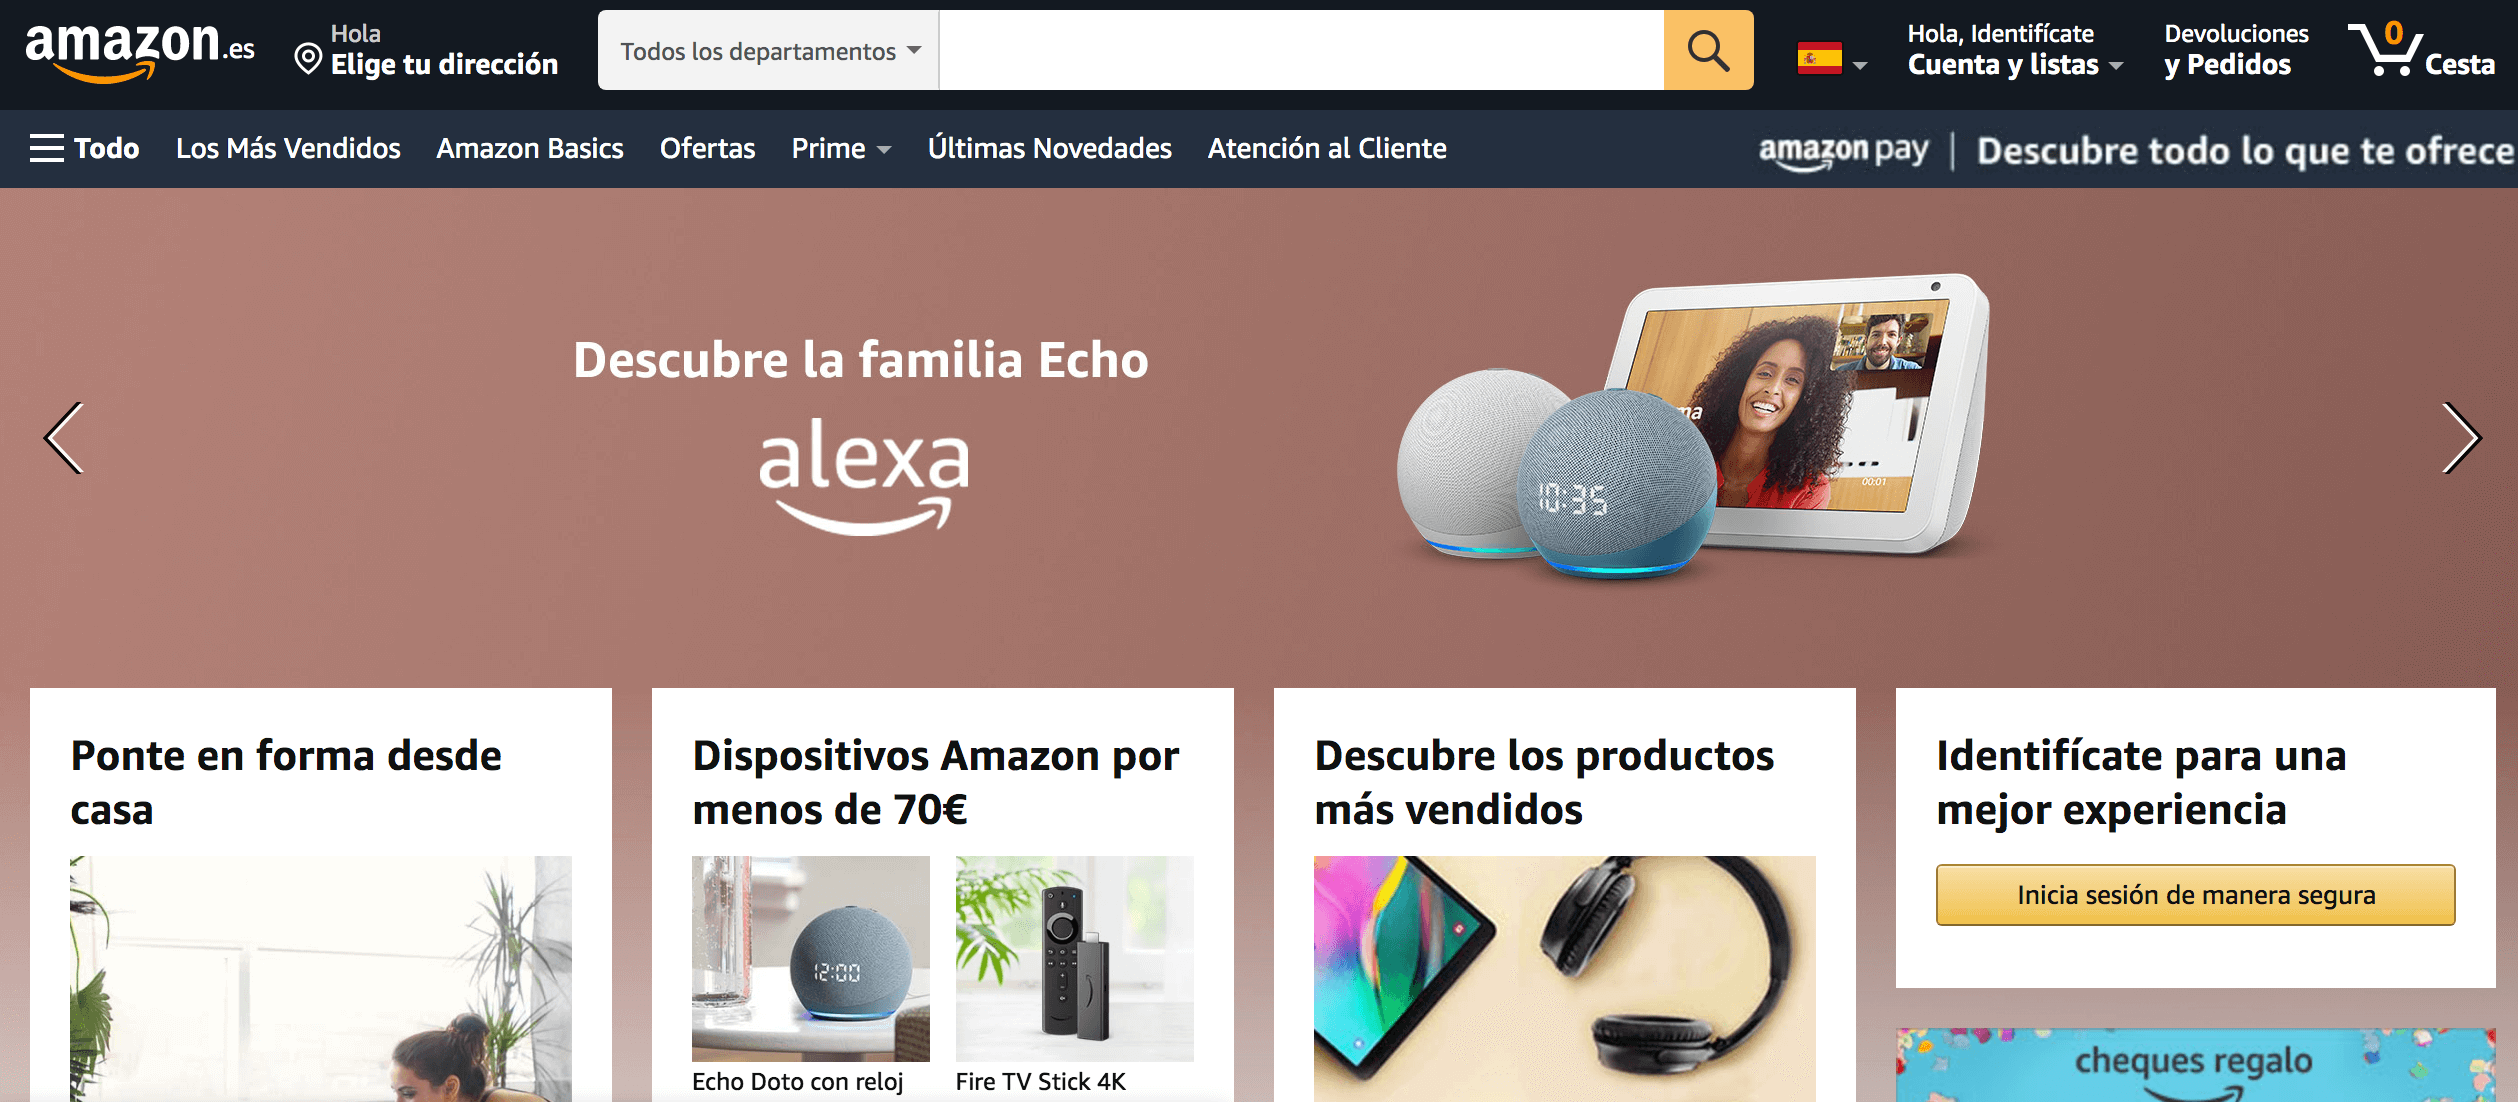
\includegraphics[width=.8\linewidth]{chapters/images/amazon.png}
  \caption{Amazon}
  \label{fig:sub-first}
\end{subfigure}
\begin{subfigure}{.5\textwidth}
  \centering
  % include second image
  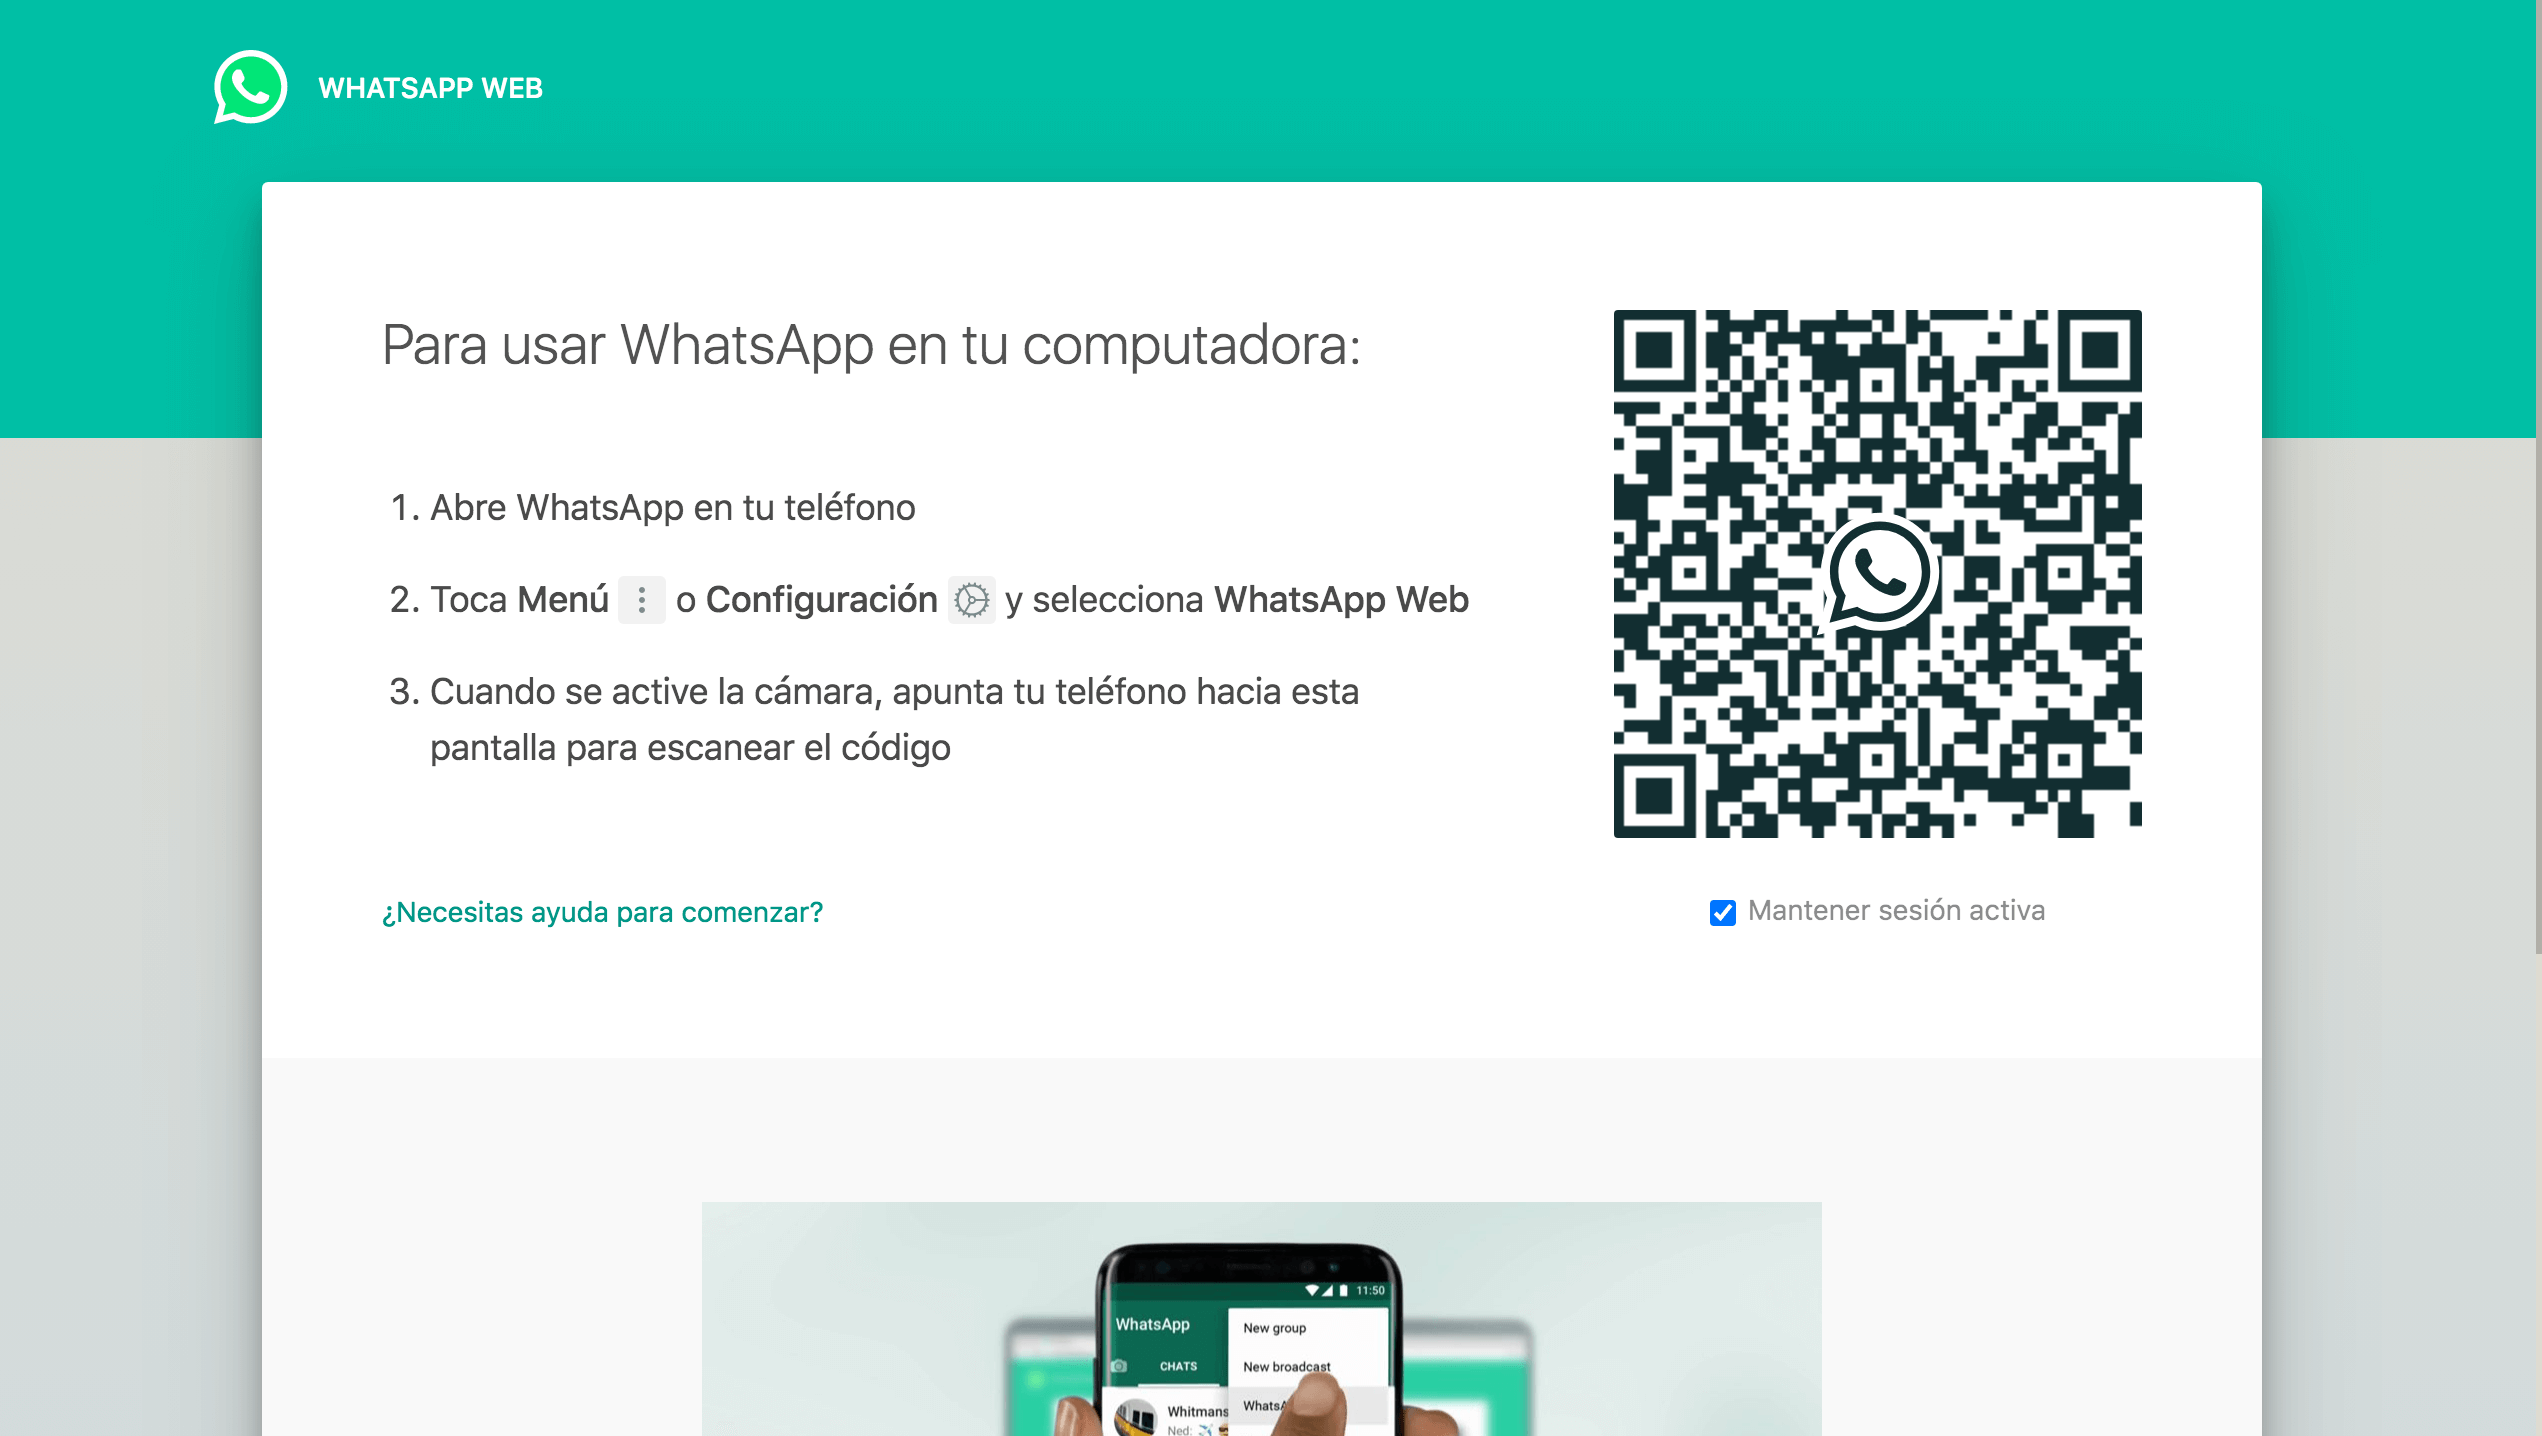
\includegraphics[width=.8\linewidth]{chapters/images/whatsappweb.png}  
  \caption{Whatsapp Web}
  \label{fig:sub-second}
\end{subfigure}
\begin{subfigure}{.5\textwidth}
  \centering
  % include third image
  
\includegraphics[width=.8\linewidth]{chapters/images/disney.jpeg}  
  \caption{Disney+}
  \label{fig:sub-third}
\end{subfigure}
\begin{subfigure}{.5\textwidth}
  \centering
  % include fourth image
  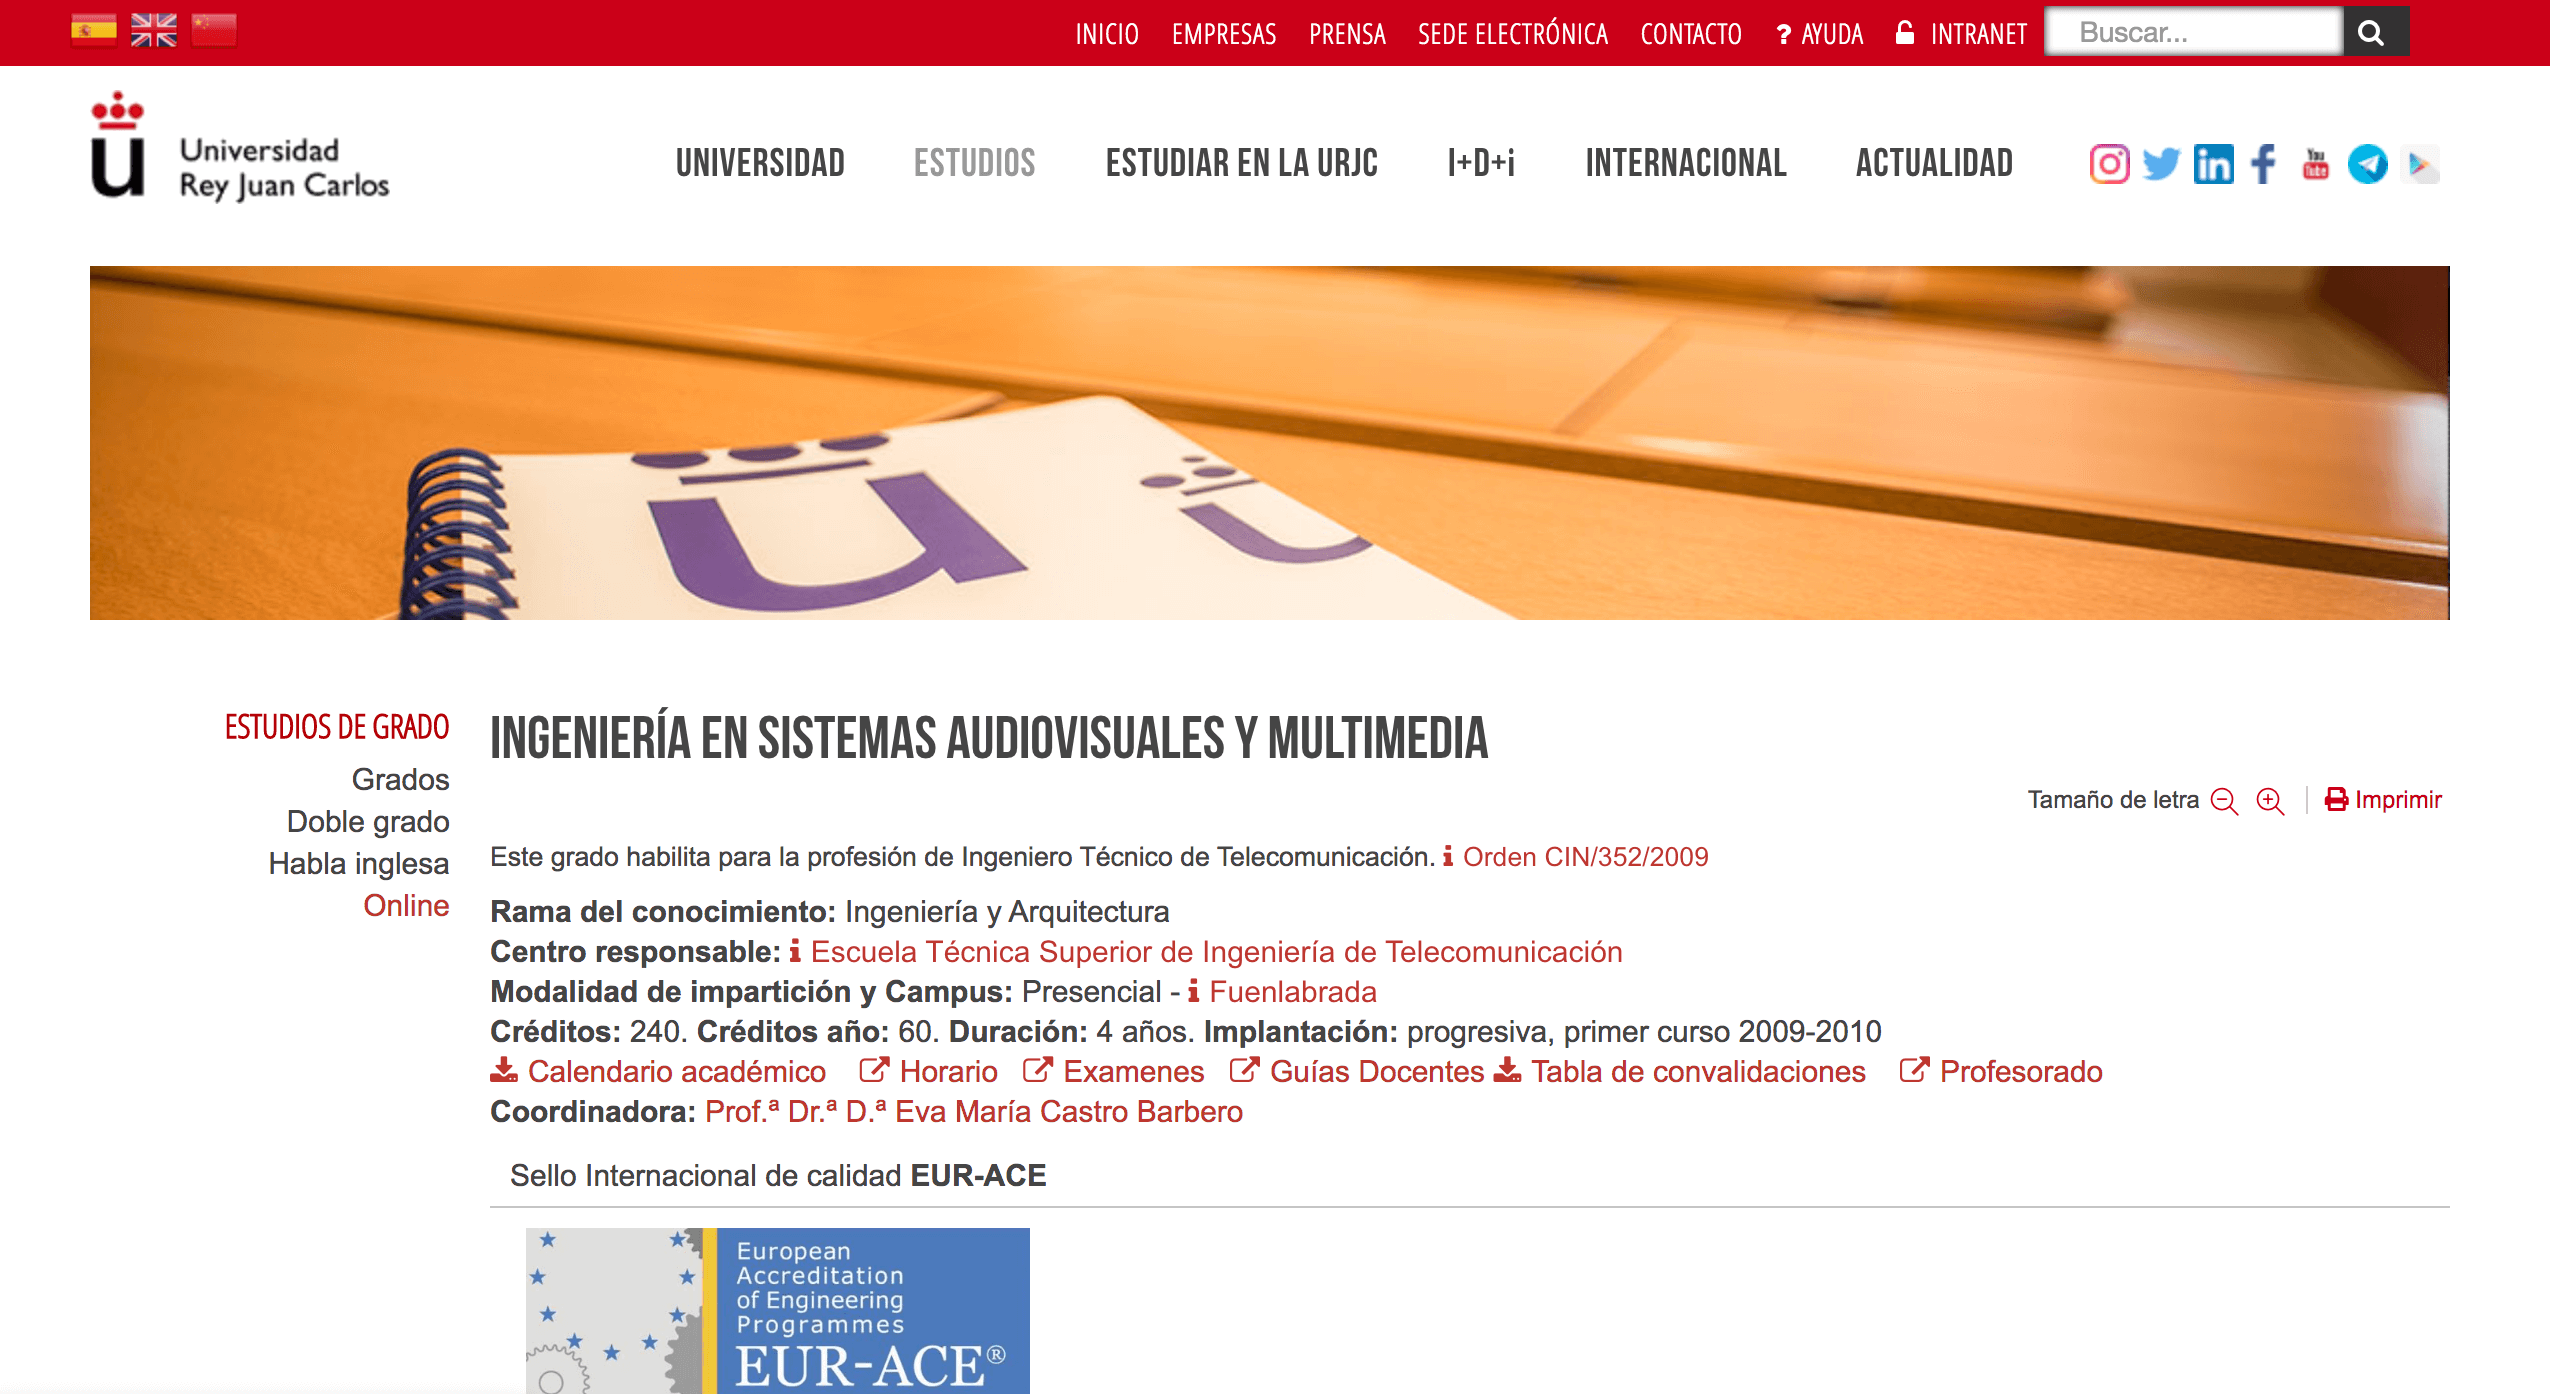
\includegraphics[width=.8\linewidth]{chapters/images/urjcweb.png}  
  \caption{URJC}
  \label{fig:sub-fourth}
\end{subfigure}
\caption{Ejemplos aplicaciones web}
\label{fig:partes robot}
\end{figure}

La web es una colección de documentos enlazados a través de hiperenlaces, cada recurso queda definido por su URL \footnote{Uniform Resource Locator}. Cuando accedemos a la web a través del navegador, tenemos que introducir la dirección URL del sitio web al que nos queremos dirigir. El navegador enviará una solicitud al servidor con el protocolo HTTP \footnote{Hyper Text Transfer Protocol}. El servidor le enviará a nuestro navegador un fichero HTML que quedará almacenado en nuestra máquina. Una vez el navegador obtiene el fichero HTML mostrará al usuario la página web principal de la URL que ha introducido. Si el navegador detecta que hay imágenes, vídeos u otros ficheros, volverá a mandar peticiones HTTP al servidor para que éste le envíe toda la información necesaria. En la Figura 1.8 podemos ver una representación de cómo es la comunicación entre cliente y servidor.
\begin{figure}[H]
    \centering
    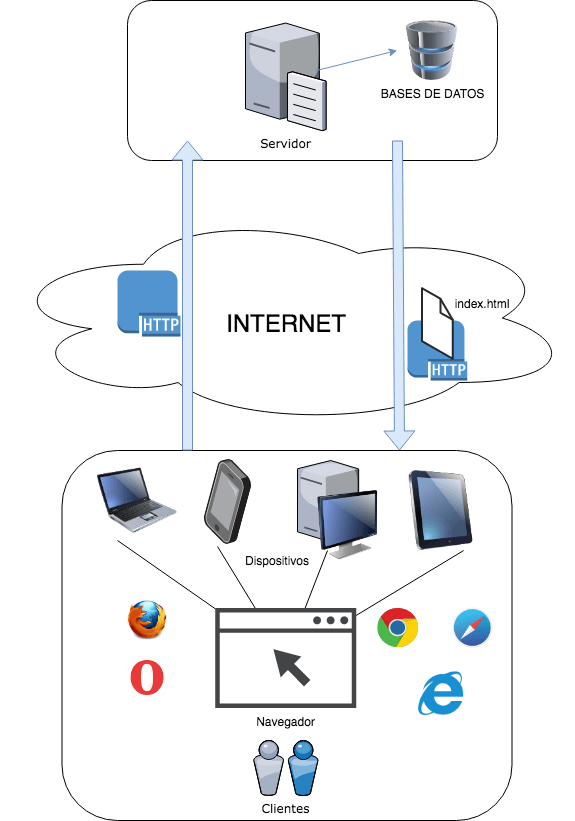
\includegraphics[width=0.45\columnwidth]{chapters/images/web.png}
    \caption{Comunicación cliente/servidor a través de HTTP}
    \label{fig:httpprotocol}
\end{figure}
 HTTP es un protocolo entre navegadores y servidores web para transferir documentos de hipertexto. El cliente envía mensajes de solicitud y el servidor manda mensajes de respuesta, ambos mensajes son del mismo formato (ver Figura 1.9 y Figura 1.10.) Los tipos de mensaje más comunes de este protocolo son GET, POST, PUT, DELETE y HEAD. Este protocolo utiliza códigos de estado, los más conocidos son: 200 OK, que significa resultado exitoso, 500 Server Error, cuando hay un error en el lado servidor y el más conocido 404 Not Found, cuando hay un error en la parte cliente. \cite{tecnologiasweb}

\begin{figure}[H]
\centering
\begin{minipage}[t]{.45\linewidth}
\centering
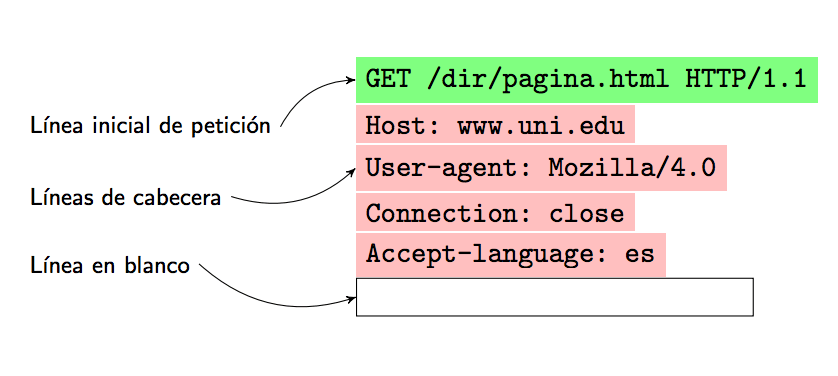
\includegraphics[width=1\columnwidth]{chapters/images/peticionhttp.png}
\caption{Ejemplo petición HTTP\\ Cliente a Servidor}
\end{minipage}
\hspace{0.25in}
\begin{minipage}[t]{.45\linewidth}
\centering
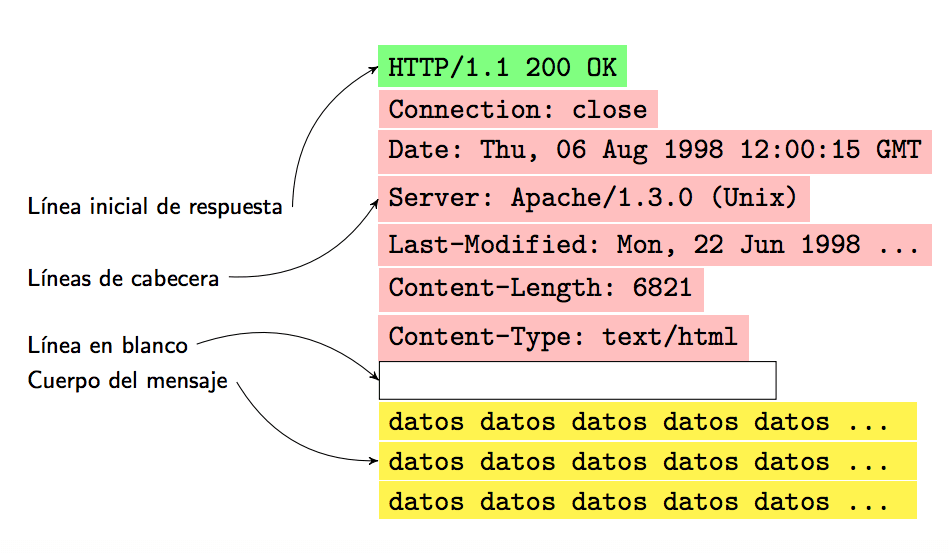
\includegraphics[width=1\columnwidth]{chapters/images/respuestahttp.png}
\caption{Ejemplo respuesta HTTP\\ Servidor a Cliente}
\end{minipage}
\end{figure}


Las dos partes que forman una aplicación web son independientes entre sí. Las tecnologías del  lado cliente (\textit{frontend}) se encargan de  interactuar con el usuario, visualizar el contenido y establecer la comunicación con el servidor. Se ejecutan en el navegador, que actúa como intérprete. Por otro lado, las tecnologías del lado servidor (\textit{backend}) se encargan de la administración del sitio web, usando bases de datos y gestores de contenidos.

Una de las principales ventajas de usar tecnologías web es que las aplicaciones creadas son multiplataforma y multidispositivo, funcionan tanto en ordenadores, móviles, tabletas, así como en distintos sistemas operativos. Otra ventaja es que no tenemos que instalar nada solo necesitamos el navegador y además la actualización del contenido es inmediata. El principal inconveniente es su dependencia de Internet, pero con los últimos avances tecnológicos el Wifi, la fibra óptica y el 5G han permitido que  mayoría de personas del mundo podamos acceder desde cualquier lugar y éste no sea un gran inconveniente.


\subsection{Tecnologías Web lado cliente}
Las tecnologías web del lado cliente  permiten la interacción del usuario con la página web que corre en el navegador del usuario. Para ello, se usan principalmente estas tres tecnologías \cite{tecnologiascliente}:

\begin{itemize}
  \item HTML5 \footnote{HyperText Markup Language}: es un lenguaje de marcado de los contenidos de un sitio web, se usa para asignar la función de cada elemento. Es el esqueleto de la web.
  \item JavaScript: es un lenguaje de programación interpretado que se encarga del comportamiento de una página web y de su interactividad con el usuario.
  \item CSS3\footnote{Cascading Style Sheets}: es un lenguaje de hojas de estilo creado para controlar la presentacion de la página: colores, tipo de letra, tamaños, animaciones, colocación de los elementos...
\end{itemize}

Entraremos en más detalle en estas tecnologías en el capítulo 3 donde se habla de la Infraestructura utilizada.

\newpage
\subsection{Tecnologías Web lado servidor}
Las tecnologías web del lado servidor son las que permiten gestionar y servir las páginas web y acceder a bases de datos. En este caso las tecnologías son más flexibles y vamos a nombrar tres de las más utilizadas:

\begin{itemize}
    \item Django: es un entorno para crear servidores web de alto nivel, que fomenta el desarrollo rápido con un diseño limpio y práctico en Python, destaca por su arquitectura basada en  modelo-vista-controlador y el uso de plantillas. De esta forma puedes centrarte en crear tu aplicacion web sin grandes complicaciones. Es gratis y de código abierto\cite{django}. Un ejemplo de aplicación web que utiliza Django es Instagram \cite{insta}.
    \item Node.js: es un entorno de ejecución para JavaScript orientado a eventos síncronos, construido con el motor de JavaScript V8 de Chrome. Diseñado para aplicaciones web escalables. De esta forma el cliente y el sevidor pueden crearse con el mismo lenguaje de programación\cite{node}. Netflix, Paypal o LinkedIn usan esta tecnología para sus servidores\cite{nodenetflix}. 
    
    \item PHP\footnote{Hypertext Preprocessor}: es un lenguaje de scripting de uso general popular que es especialmente adecuado para el desarrollo web\cite{php1}. Rápido, flexible y práctico, gracias a su capacidad de creación de webs dinámicas, desde blogs hasta sitios web como Facebook o Wikipedia\cite{php2}.
    
\end{itemize}

En el lado servidor se utilizan bases de datos. Una base de datos es una colección de datos estructurados. Entre ellas podemos destacar mySQL(Figura 1.11a) y MongoDB(Figura 1.11 b). 

\begin{figure}[H]
  \begin{subfigure}[b]{0.5\textwidth}
  \centering
    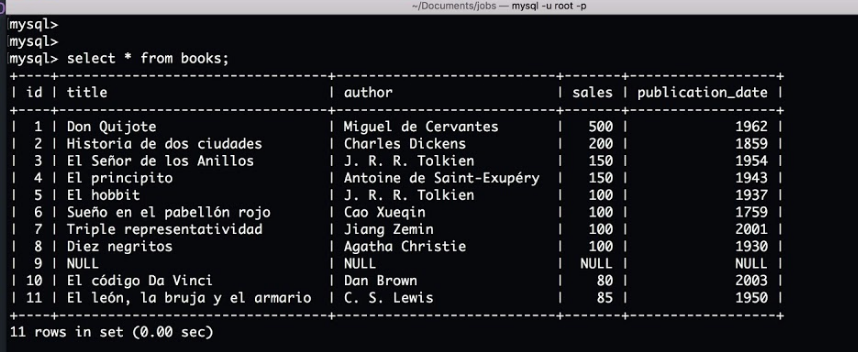
\includegraphics[width=1\textwidth, height=0.7\textwidth]{chapters/images/mysql.png}
    \caption{mySQL}
    \label{fig:f1}
  \end{subfigure}
  \hfill
  \begin{subfigure}[b]{0.5\textwidth}
  \centering
    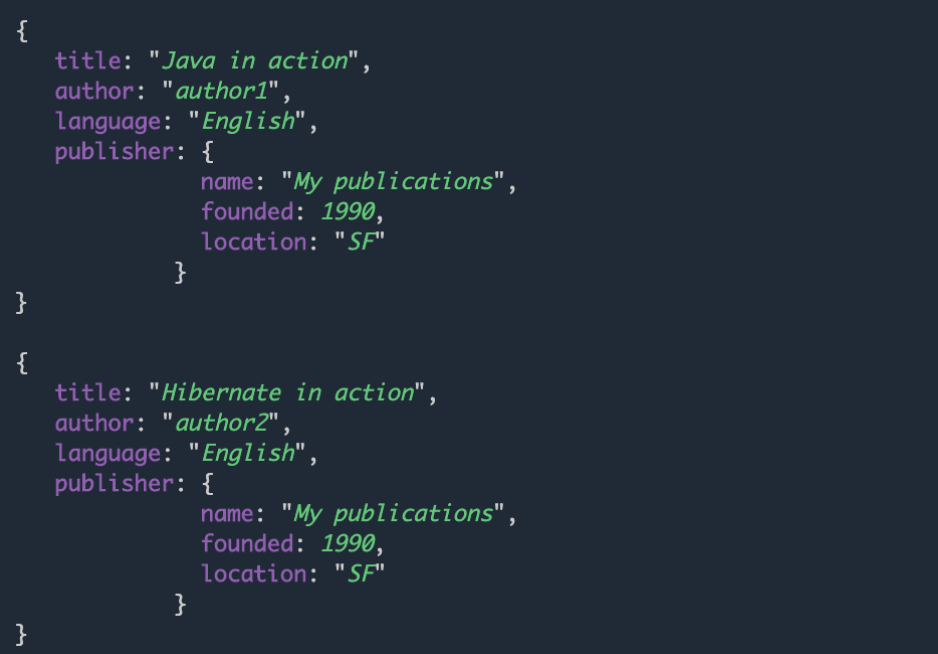
\includegraphics[width=1\textwidth, height=0.7\textwidth]{chapters/images/mongodb.png}
    \caption{MongoDB}
    \label{fig:f2}
  \end{subfigure}
  \caption{Bases de Datos}
\end{figure}



%%%%%%%%%%%%%%%%%%%%%%%%%%%%%%%%%%%%%%%%%%%%%%%%%%%%%%%%%%%%%%%%%%%%%%%%%%%%%%%%%%%%%%%%%%%%%%%%%%%%%%%%%%%%%%%%
\newpage
\section{Robótica educativa}

La Robótica educativa es un sector de aprendizaje multidisciplinar. Ayuda a desarrollar competencias y habilidades como: la innovación y espíritu emprendedor, la resolución de problemas y lógica, la toma de decisiones, conocimientos de herramientas relacionadas con las tecnologías digitales, el pensamiento crítico, creatividad, el trabajo colaborativo y cooperativo, la flexibilidad y adaptabilidad al trabajo \cite{roboticaedu}.
\\
Ante la falta de estudiantes en carreras técnicas en la actualidad, la robótica educativa puede ofrecer una gran motivación a los alumnos de las primeras etapas de educación: Primaria, ESO y Bachillerato, para fomentar la creatividad y la curiosidad al mostrar la ciencia y la tecnología de una forma diferente e incrementar sus habilidades a la vez que sus conocimientos desde los fundamentos STEM (\textit{Science, Technology, Engineering and Mathematics}).

Gracias a las tecnologías web son muchas las  aplicaciones que ofrecen cursos de robótica para todos los niveles educativos, muchos ayuntamientos están comprando cursos y materiales para facilitar a los más pequeños su introducción al mundo de la robótica a través de clases extraescolares. En secundaria se está introduciendo poco a poco en las asignaturas de tecnología el uso de lenguajes de programación, en el que destaca el lenguaje Scratch. En la Figura 1.12 podemos ver la interfaz de Scratch para programar desde el navegador.
\begin{figure}[H]
    \centering
    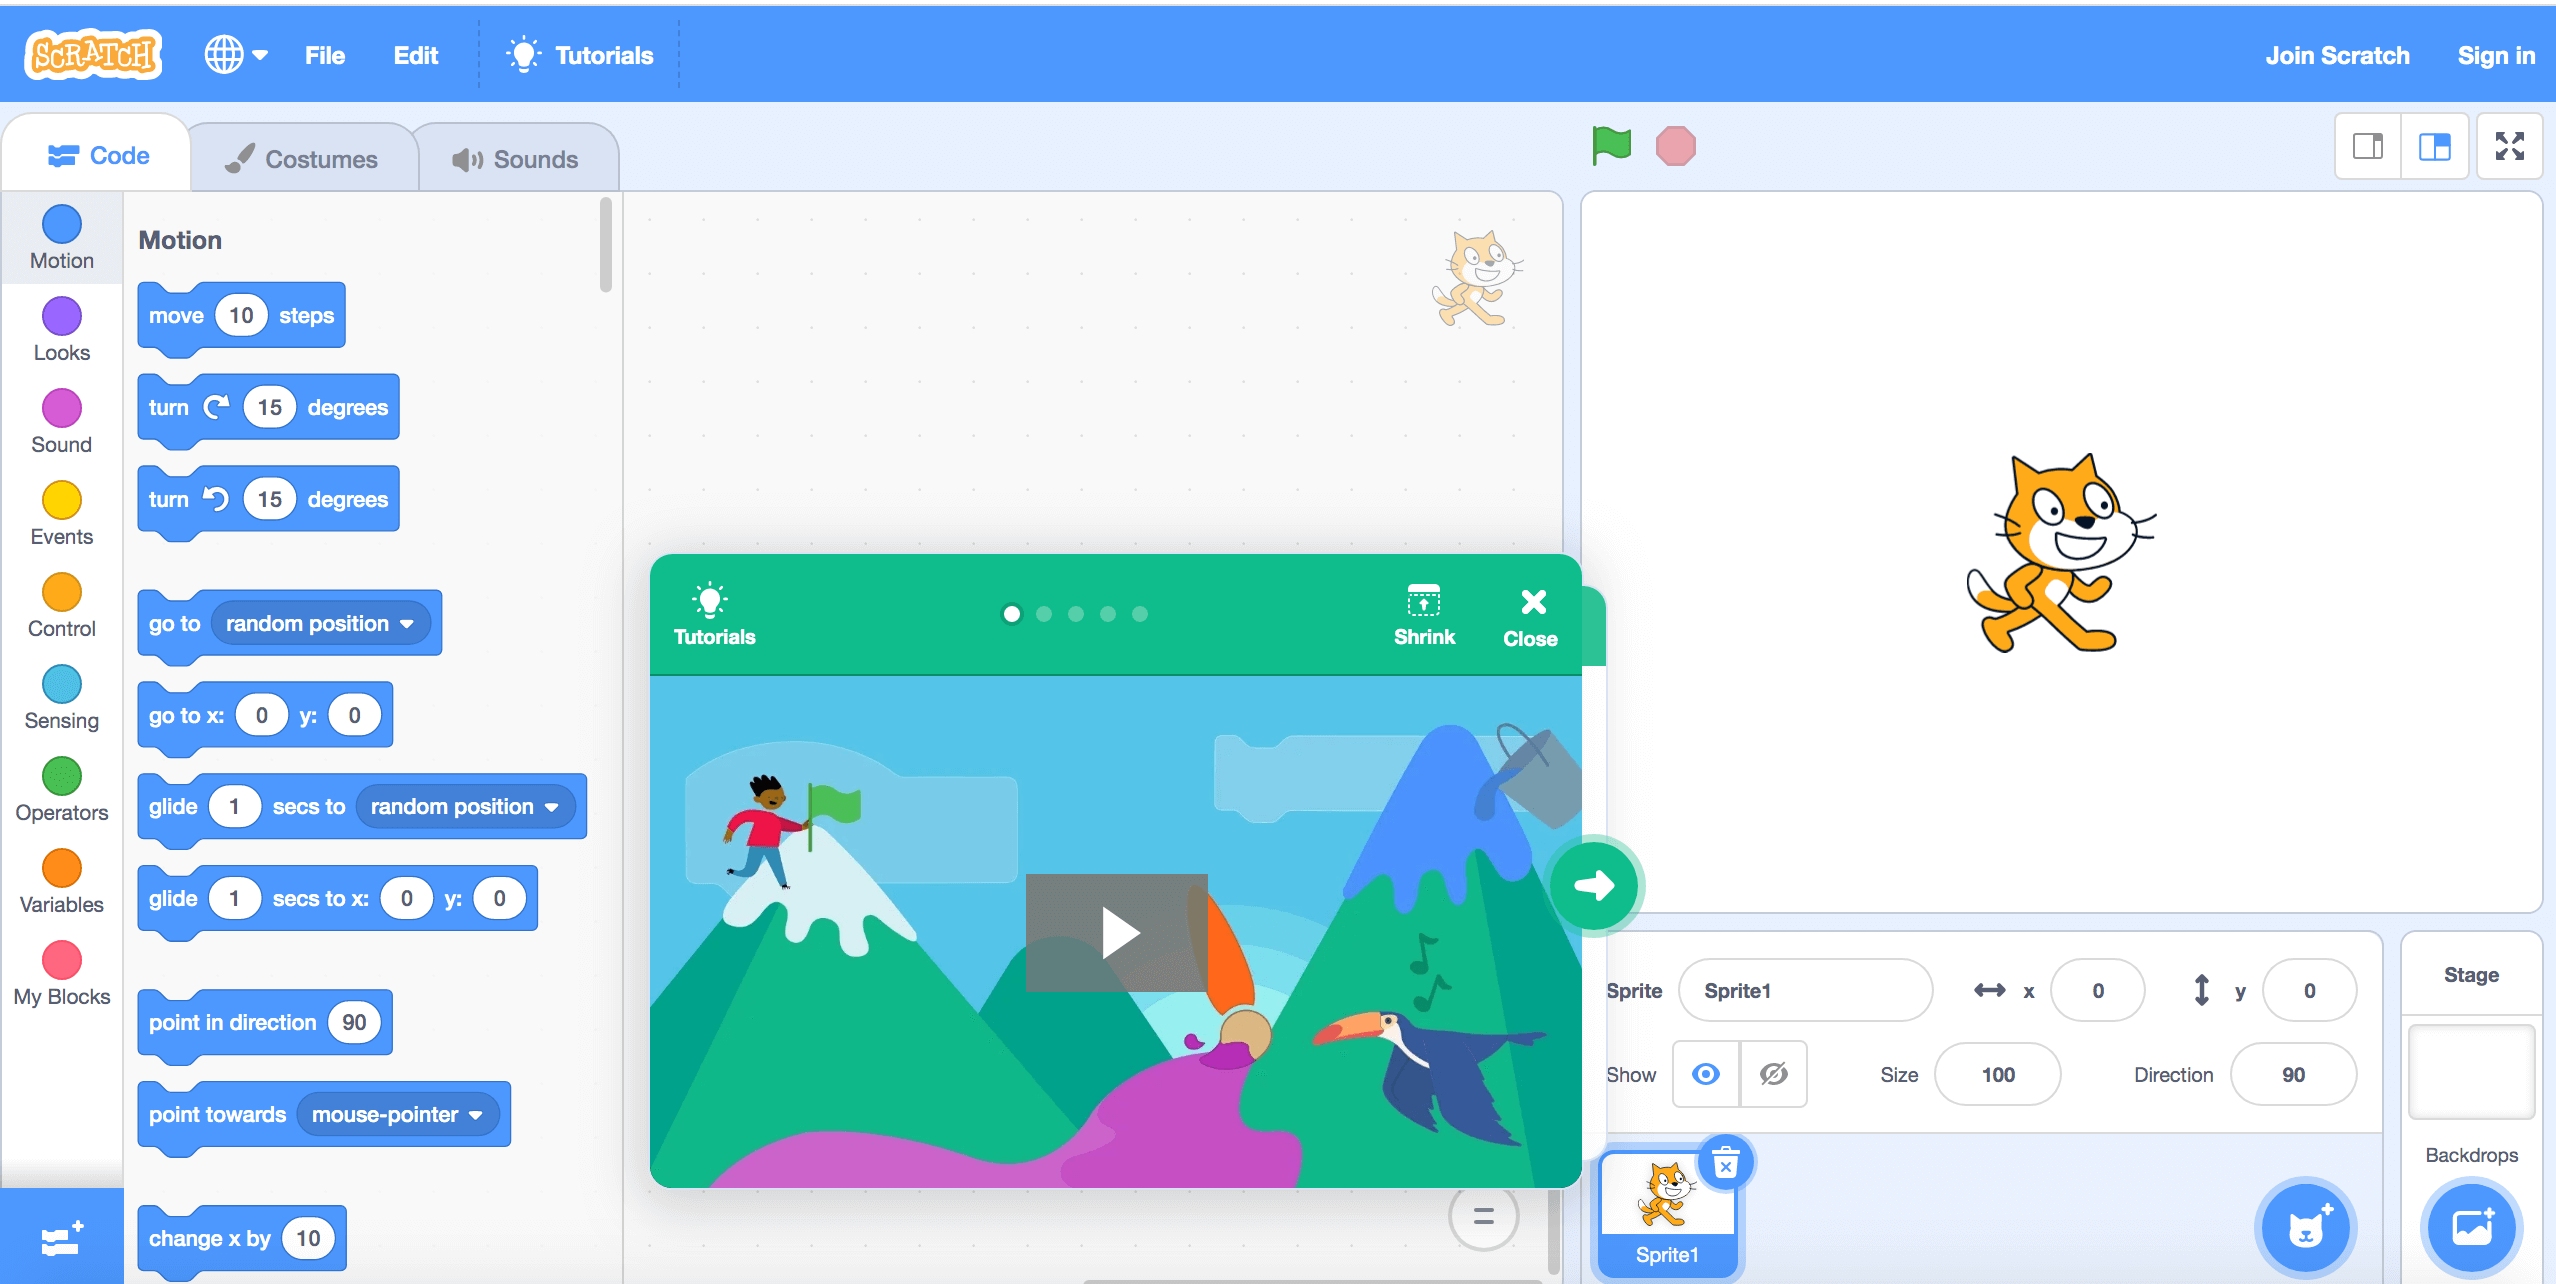
\includegraphics[width=0.8\columnwidth]{chapters/images/scratch.png}
    \caption{Scratch}
    \label{fig:my_label}
\end{figure}

Scratch es un lenguaje de programación visual basado en bloques, creado y  mantenido por Lifelong Kindergarten group en el MIT Media Lab. Scratch además es una comunidad en línea donde los niños pueden programar y compartir medios interactivos como historias, juegos y animaciones con gente de todo el mundo. Los más pequeños aprenden a pensar creativamente, trabajar en colaboración y razonar sistemáticamente\cite{scratch}. Scratch posee un lenguaje de iniciación llamado Scratch Jr pensando para niños de 5 a 7 años siendo aún más sencillo, aunque Scratch está pensado para todas las edades. Actualmente se puede utilizar desde cualquier dispositivo al ultilizar tecnologías web.

Junto con Scratch cada vez hay más plataformas y entornos STEM que se han dedicado al desarrollo de herramientas de aprendizaje enfocadas a los más pequeños. Destacan aplicaciones web como: 

\begin{itemize}
    \item  \textit{OpenRoberta \footnote{https://lab.open-roberta.org/}}: es una plataforma web creada por un instituto alemán perteneciente a la Fraunhofer Society. Tiene como objetivo simplificar conceptos de programación y facilitar a niños y profesores la codificación mediante el uso de robots como Lego Mindstorms y otros sistemas de hardware programables. \cite{openroberta}. 
    
    \begin{figure}[H]
        \centering
        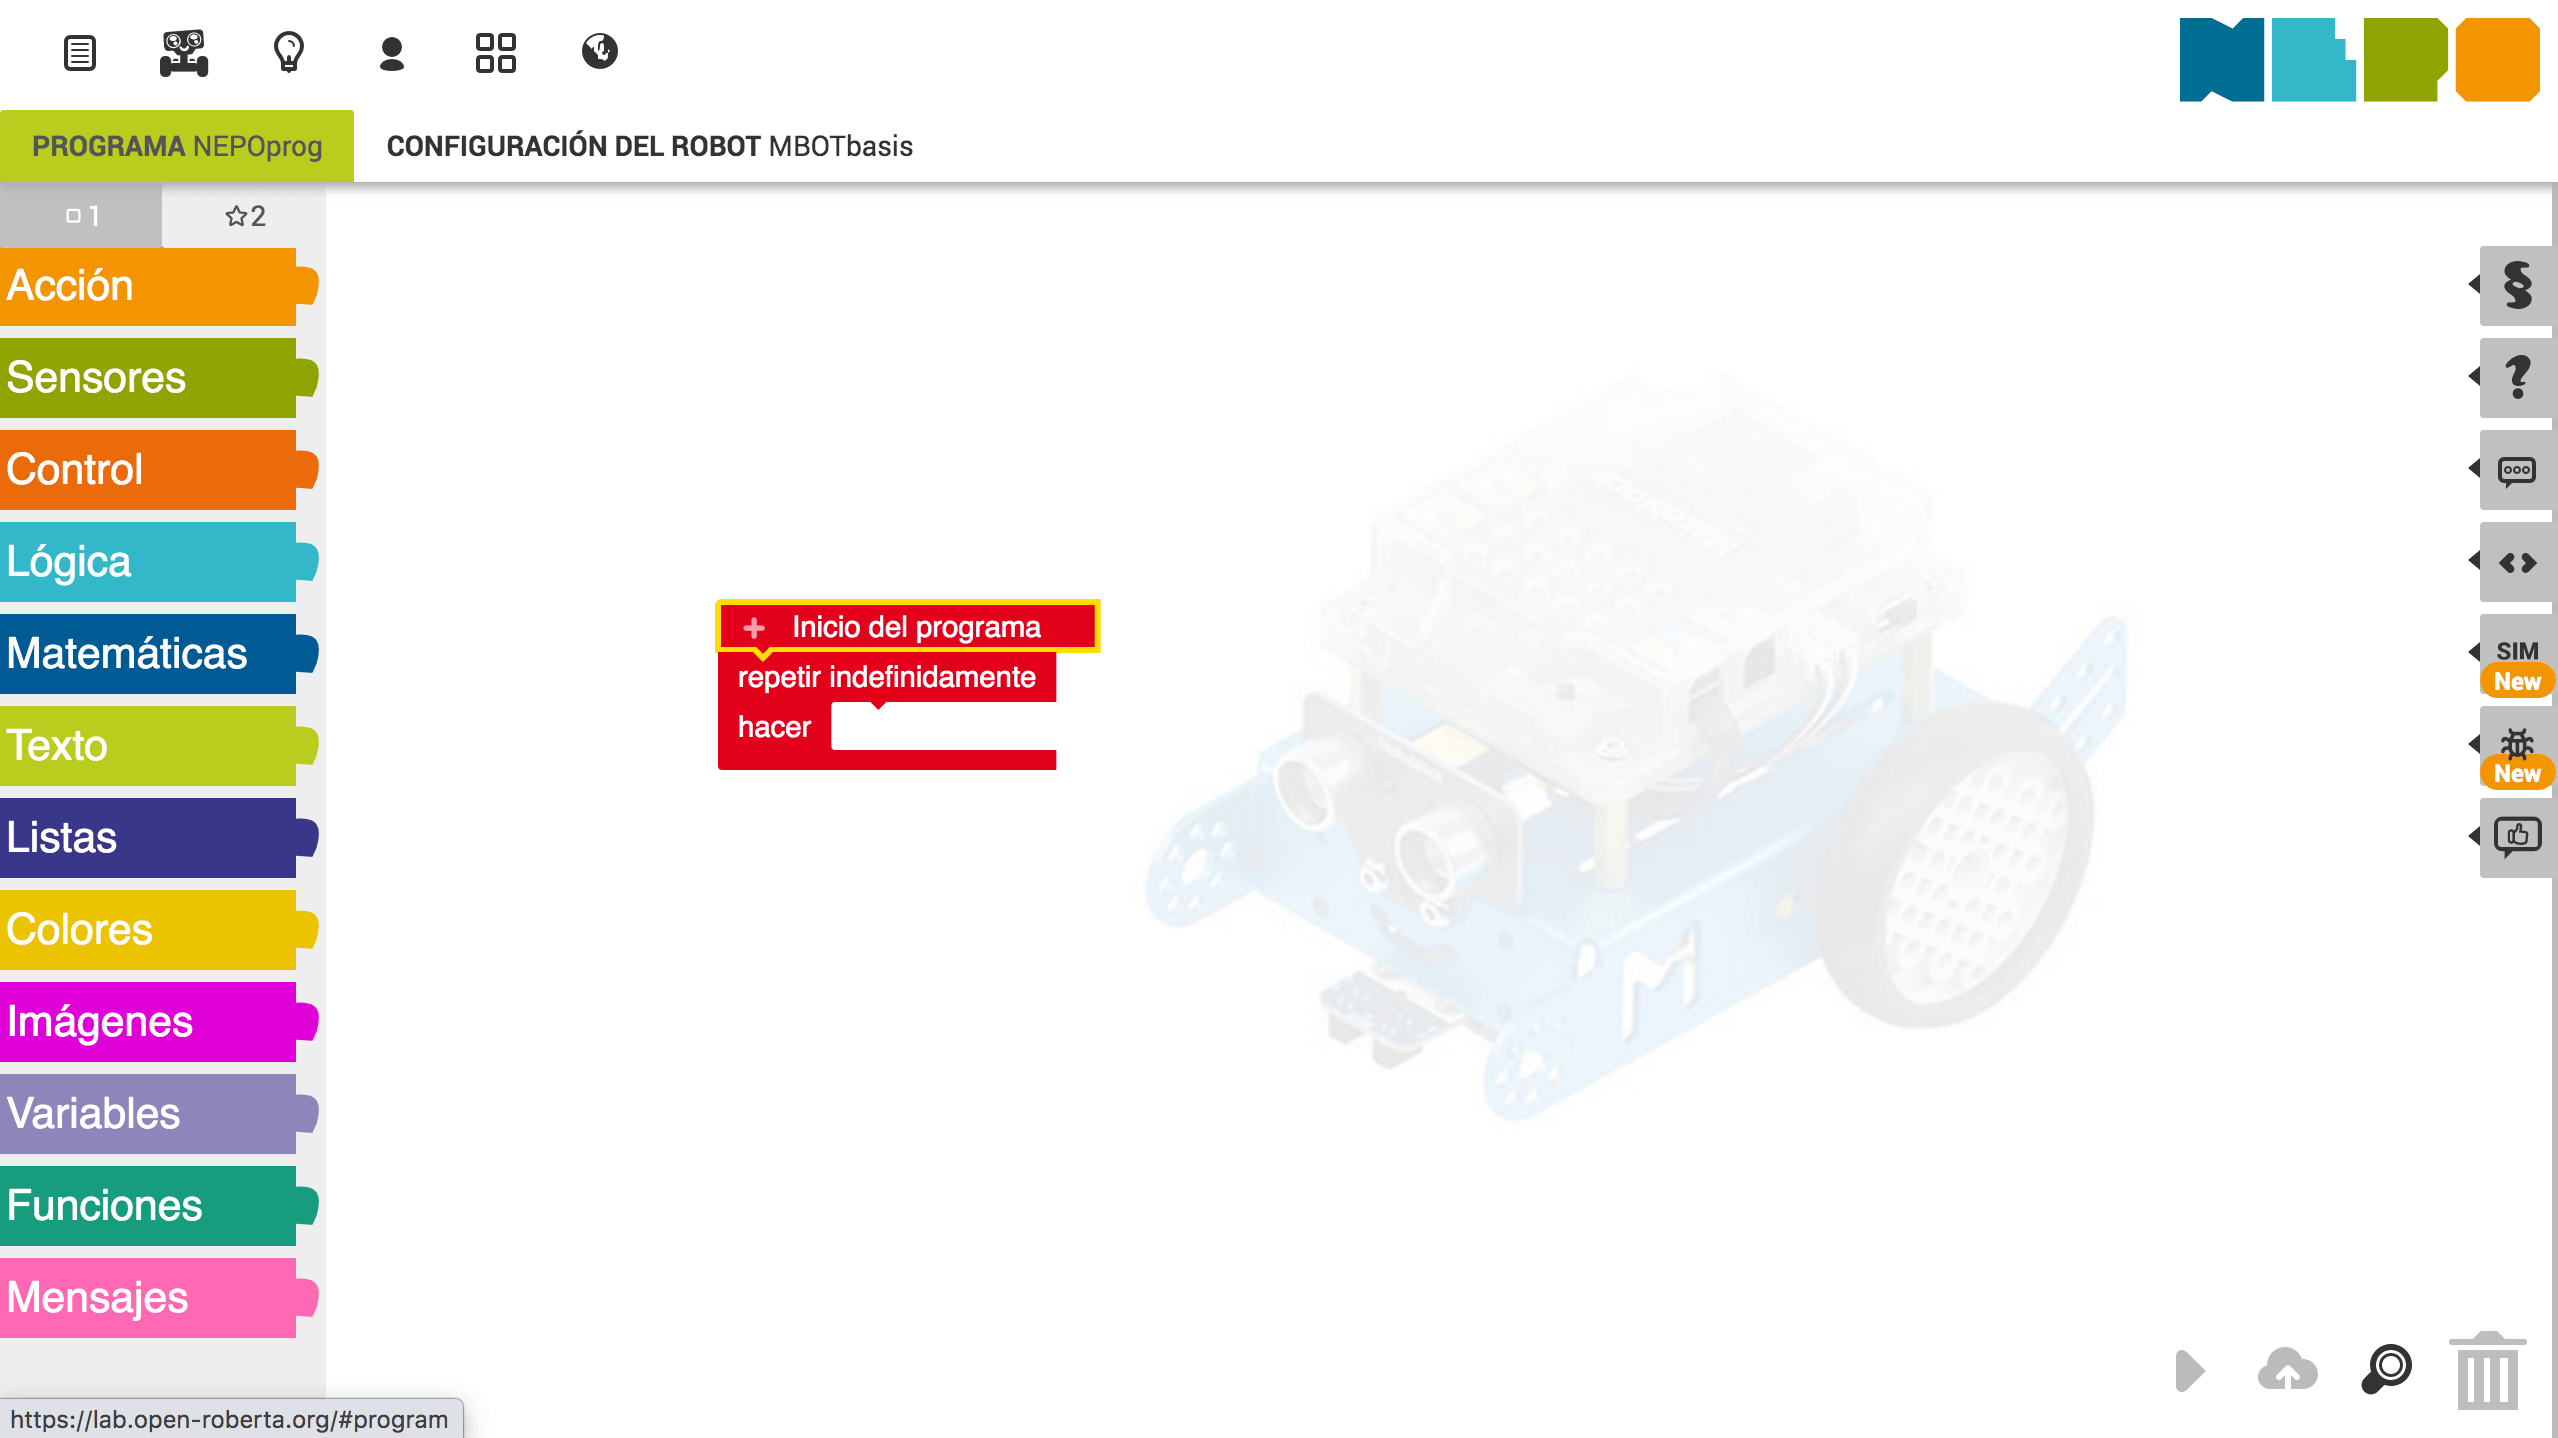
\includegraphics[width=0.7\textwidth ]{chapters/images/openrobert.png}
        \caption{Open Roberta}
        \label{fig:openroberta}
    \end{figure}
    \item \textit{LEGO Education}: la plataforma LEGO ofrece una amplia variedad de robots y \textit{packs} para uso escolar. Sus kits de robótica educativa permiten a los más pequeños construir y programar robots mediante el uso de motores, sensores, engranajes, ruedas, ejes y otros componentes técnicos, además del uso de su propio software basado en bloques. Destacan modelos como  MINDSTORMS Education EV3 y LEGO Education WeDo 2.0.\cite{ev3} \cite{legoeducation}

    \begin{figure}[H]
  \begin{subfigure}[b]{0.5\textwidth}
  \centering
    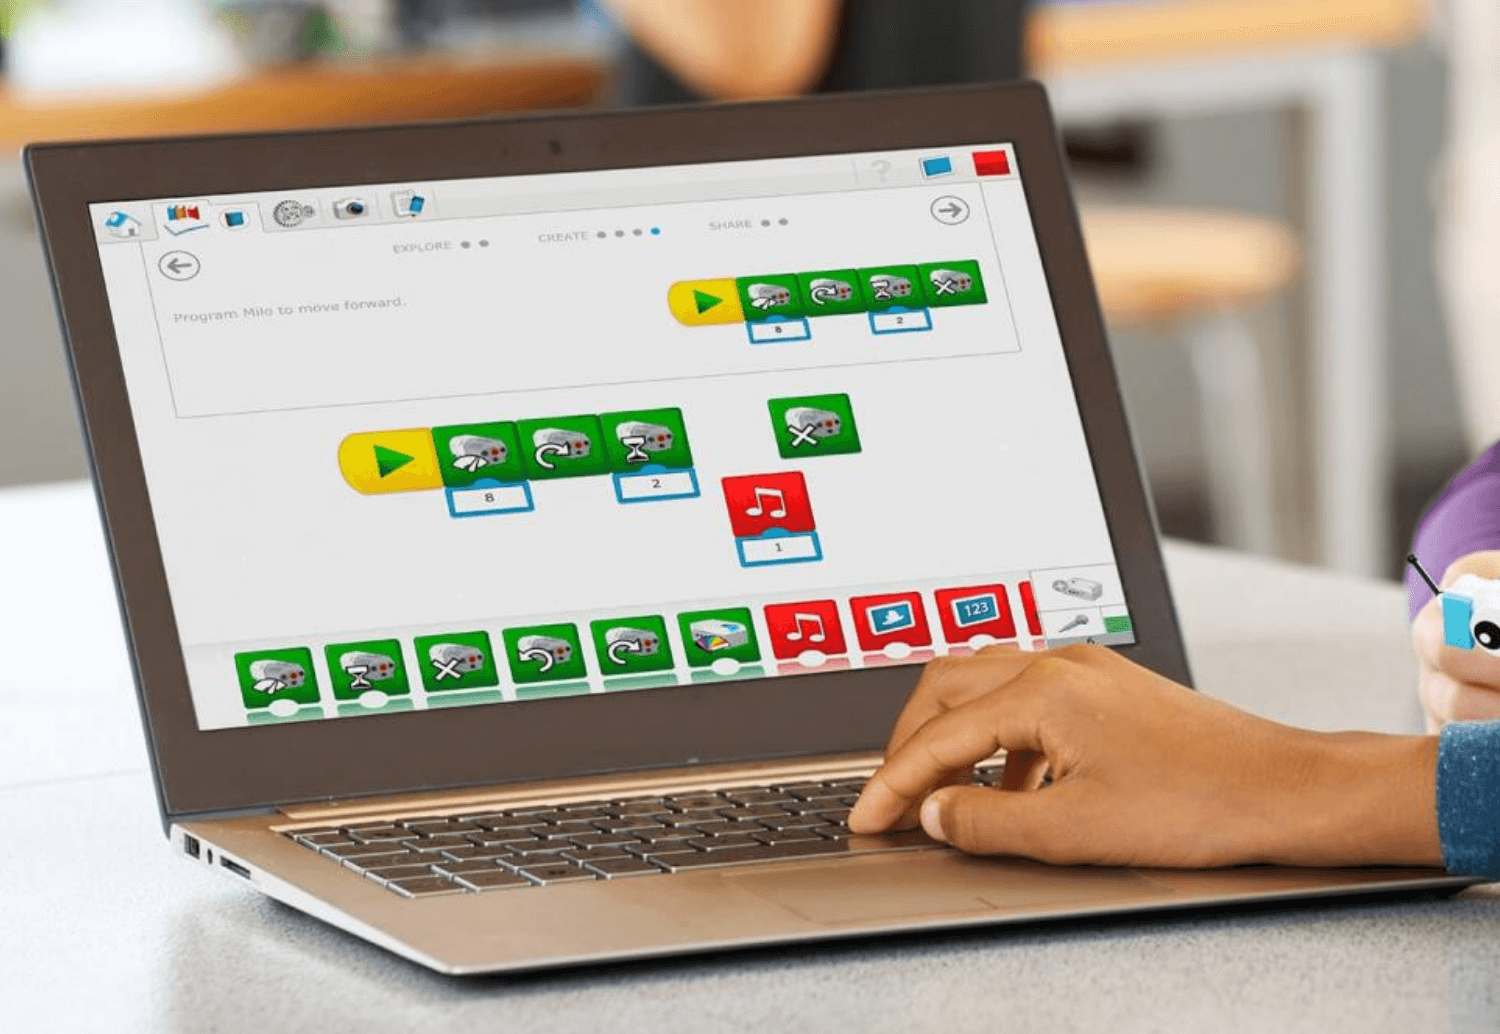
\includegraphics[width=0.9\textwidth, height=0.5\textwidth]{chapters/images/legoo.png}
    \caption{LEGO}
    \label{fig:f1}
  \end{subfigure}
  \hfill
  \begin{subfigure}[b]{0.5\textwidth}
  \centering
    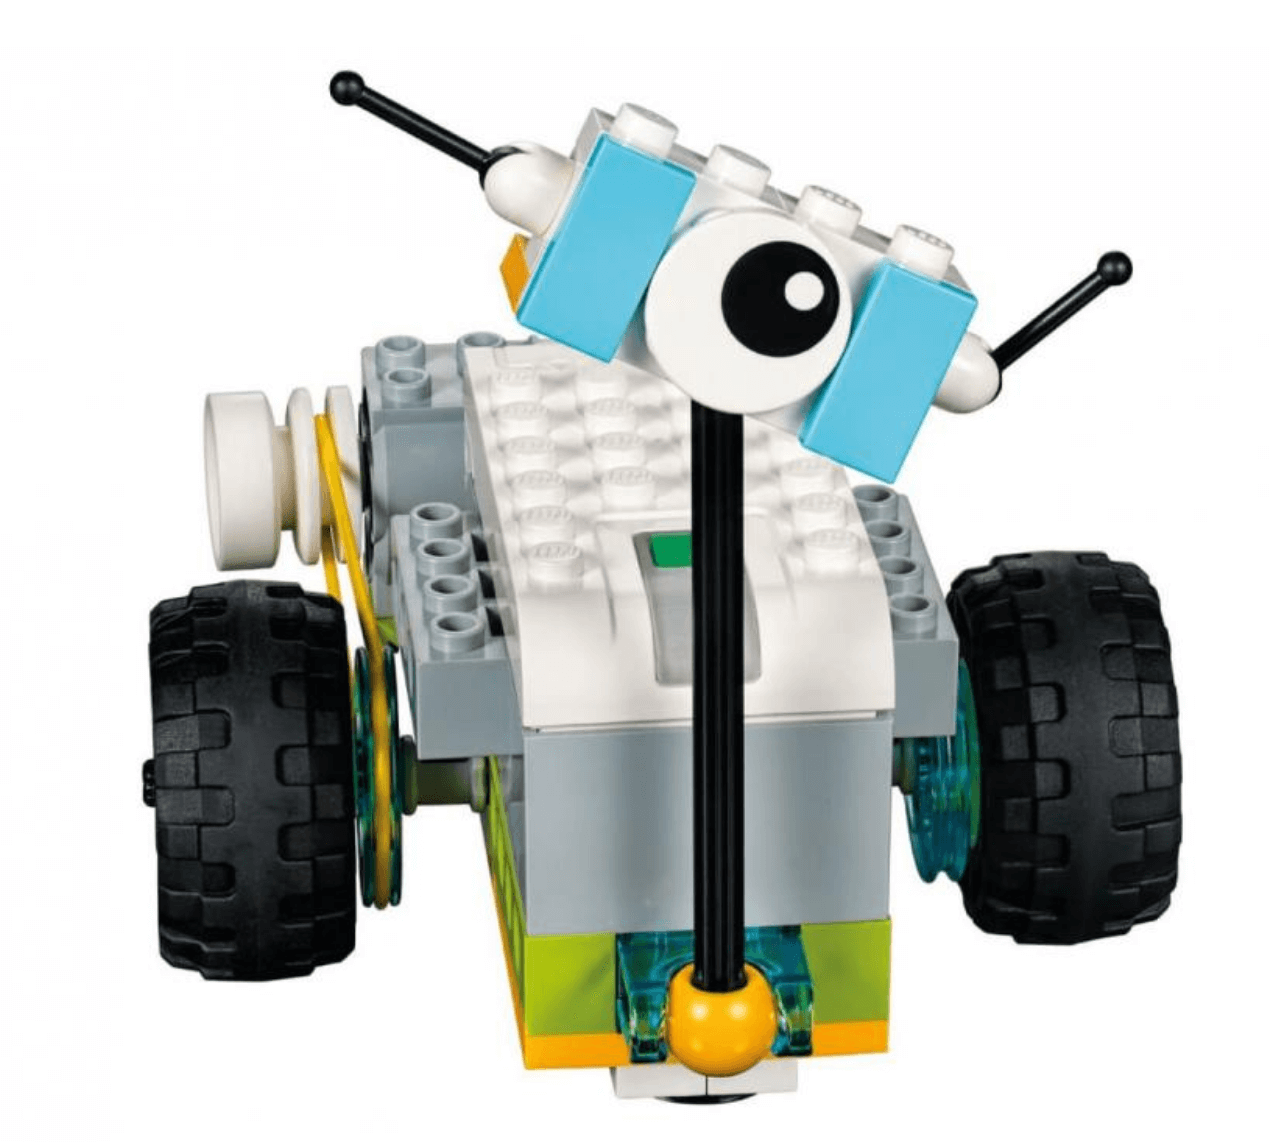
\includegraphics[width=0.9\textwidth, height=0.5\textwidth]{chapters/images/wedo.png}
    \caption{WeDo 2.0}
    \label{fig:f2}
  \end{subfigure}
  \caption{LEGO EDUCATION}
\end{figure}

    \item \textit{MBlock IDE \footnote{https://ide.mblock.cc/}}: esta aplicación web está diseñada para la educación en ciencia, tecnología, ingeniería, artes y matemáticas (STEAM). Está inspirada en Scratch 3.0, es compatible con lenguajes de programación tanto gráficos (Scratch) como textuales (Python). Se pueden diseñar historias, juegos, animaciones y programar dispositivos como robots Makeblock y microbit. \cite{mblock}
    \begin{figure}[H]
        \centering
        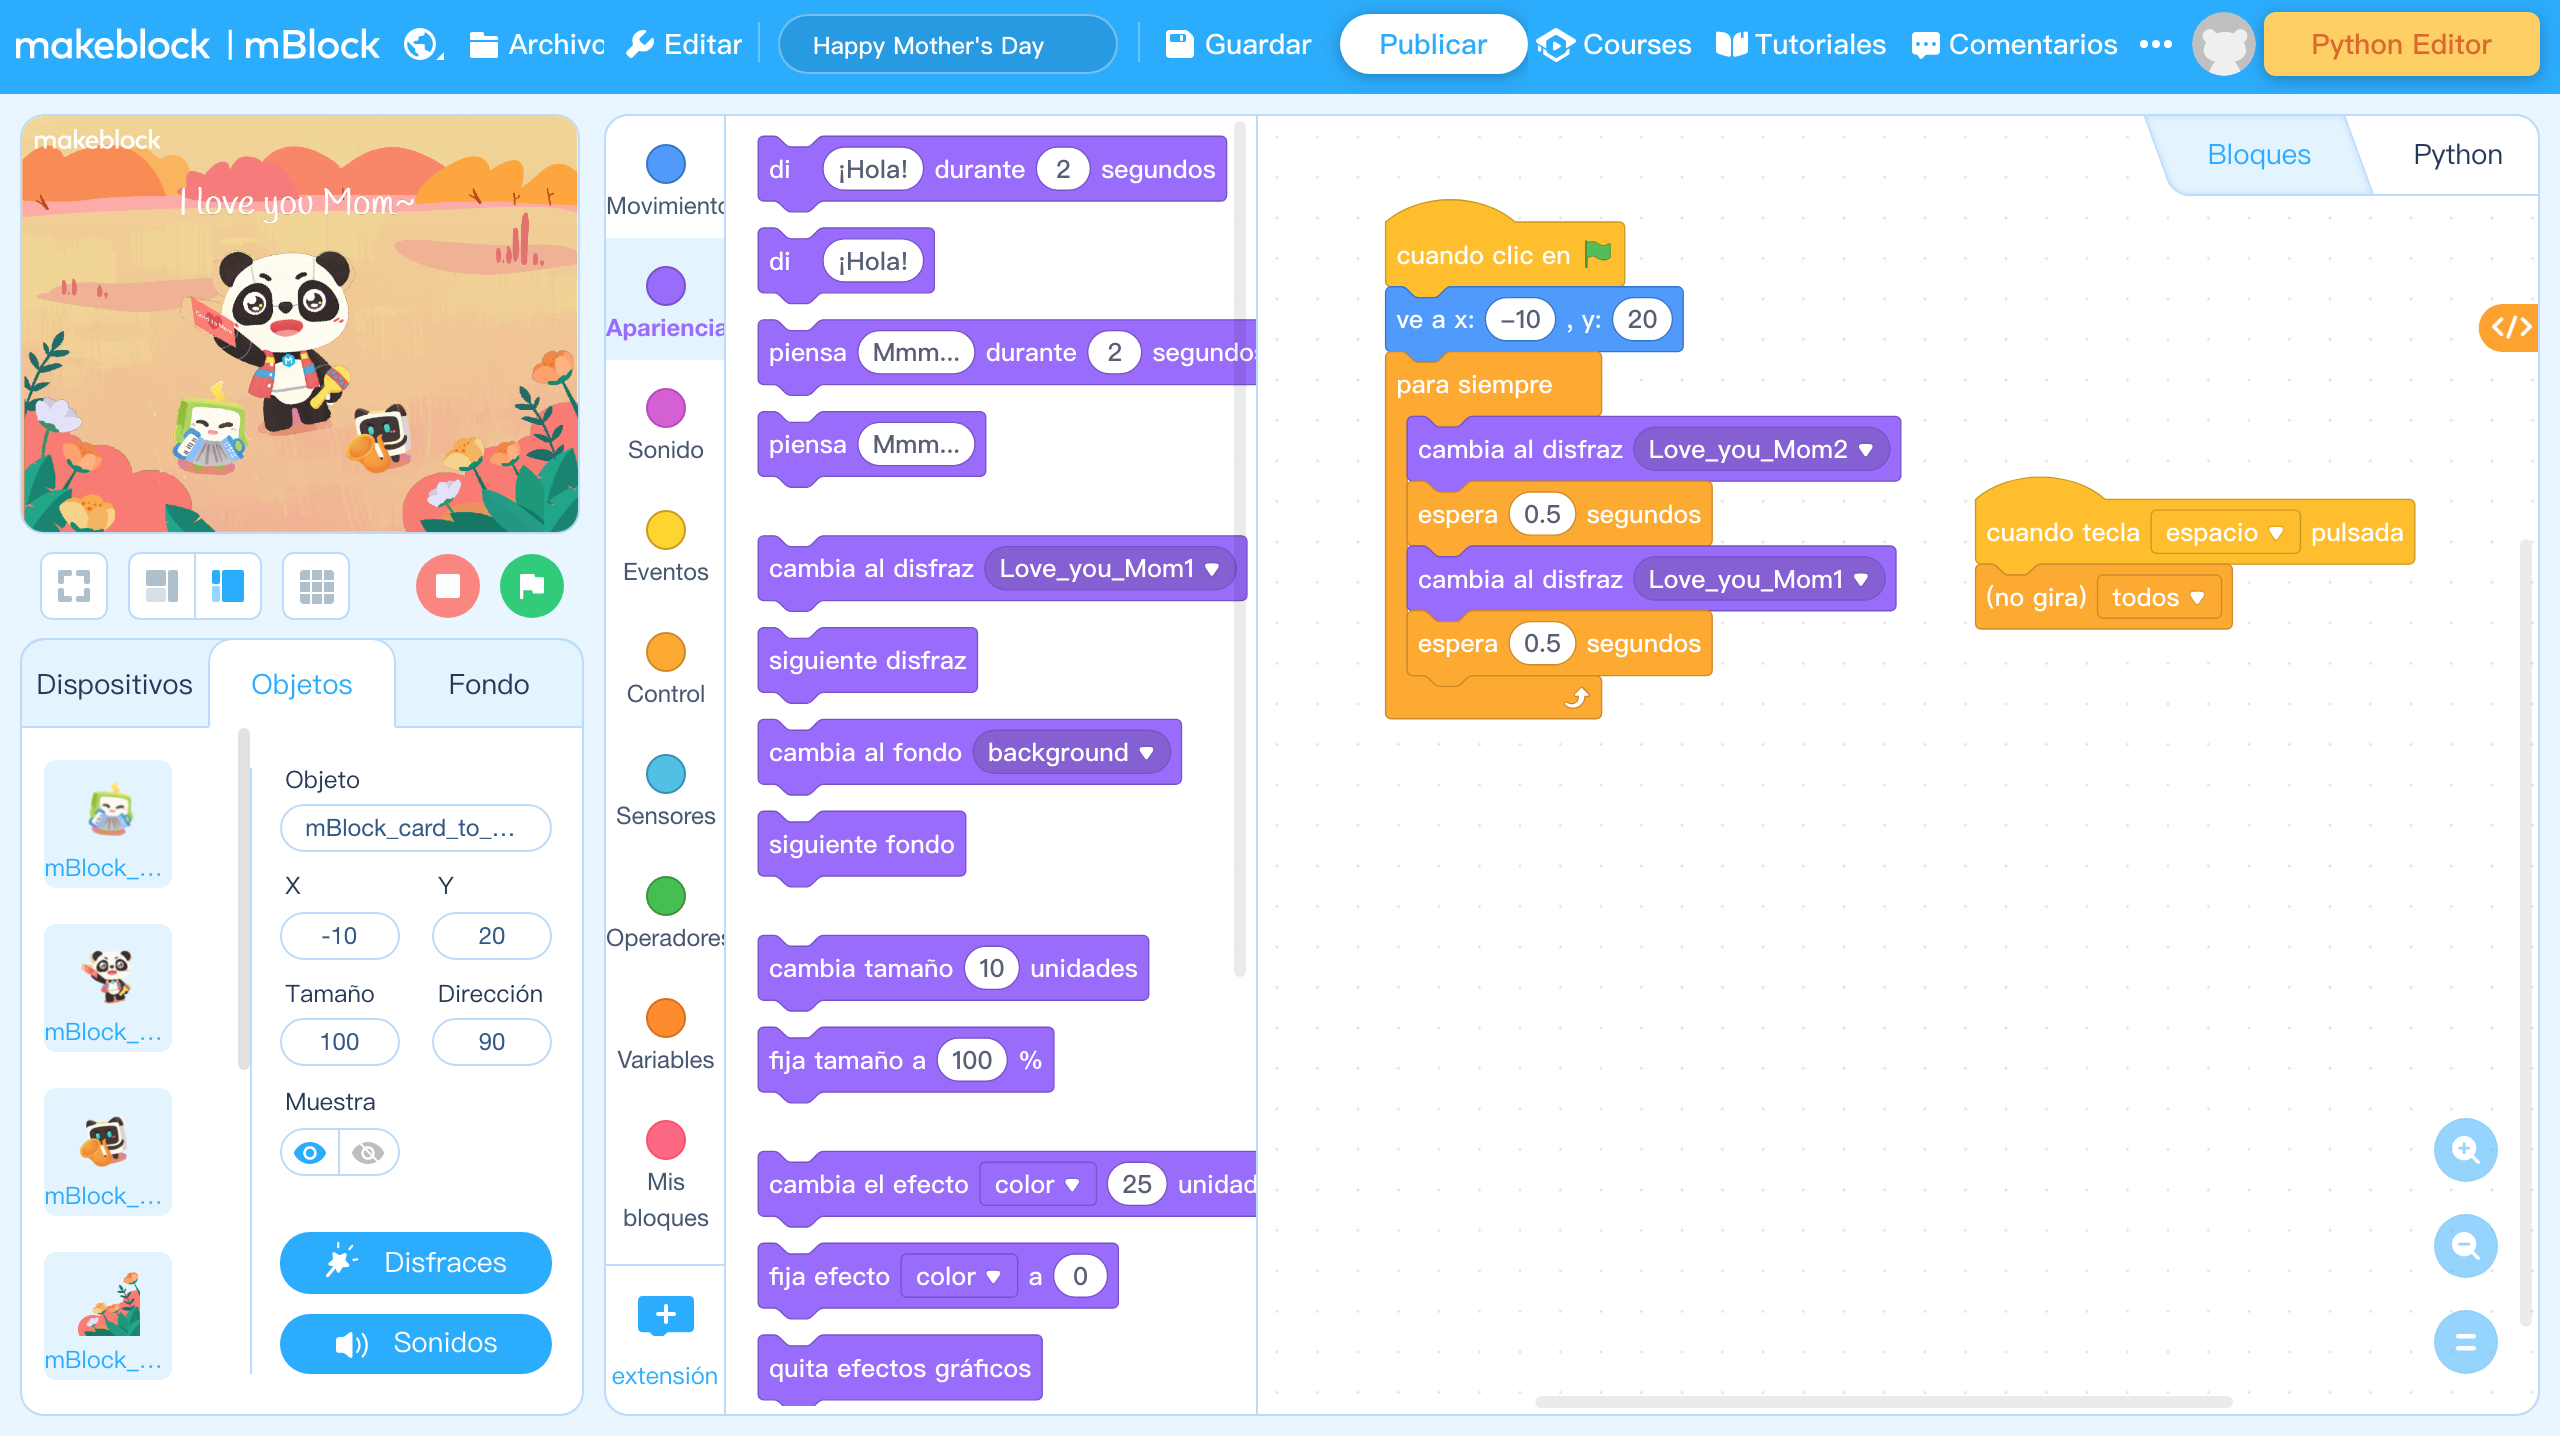
\includegraphics[width=0.7\textwidth]{chapters/images/makeblock.png}
        \caption{MBlock IDE}
        \label{fig:mblock}
    \end{figure}

    \item Vex \footnote{https://www.vexrobotics.com/}, AppInventor \footnote{https://appinventor.mit.edu/}, Arduino Web Editor\footnote{https://store.arduino.cc/digital/create}, Kodu \footnote{http://www.kodugamelab.com/} o Snap! \footnote{https://snap.berkeley.edu/} son otras plataformas web de programación en robótica educativa.
\end{itemize}


La plataforma de robótica educativa que vamos utilizar en este TFG es Kibotics. Esta plataforma, basada en tecnologías web, enseña de manera atractiva conceptos básicos de tecnología e inicia a niños y adolescentes en robótica y programación. Sigue un enfoque práctico, fomentando el pensamiento y la organización para resolver un problema. Además de formar el espíritu analítico de los alumnos \cite{intro}.
\\
Actualmente ofrece cursos de robótica en Scratch y Python (Figura 1.16). En el capítulo 3 se ampliará información sobre Kibotics y veremos cómo se introduce la \textit{Gamificación} en la plataforma a lo largo de este trabajo.

\begin{figure}[H]
  \begin{subfigure}[b]{0.5\textwidth}
  \centering
    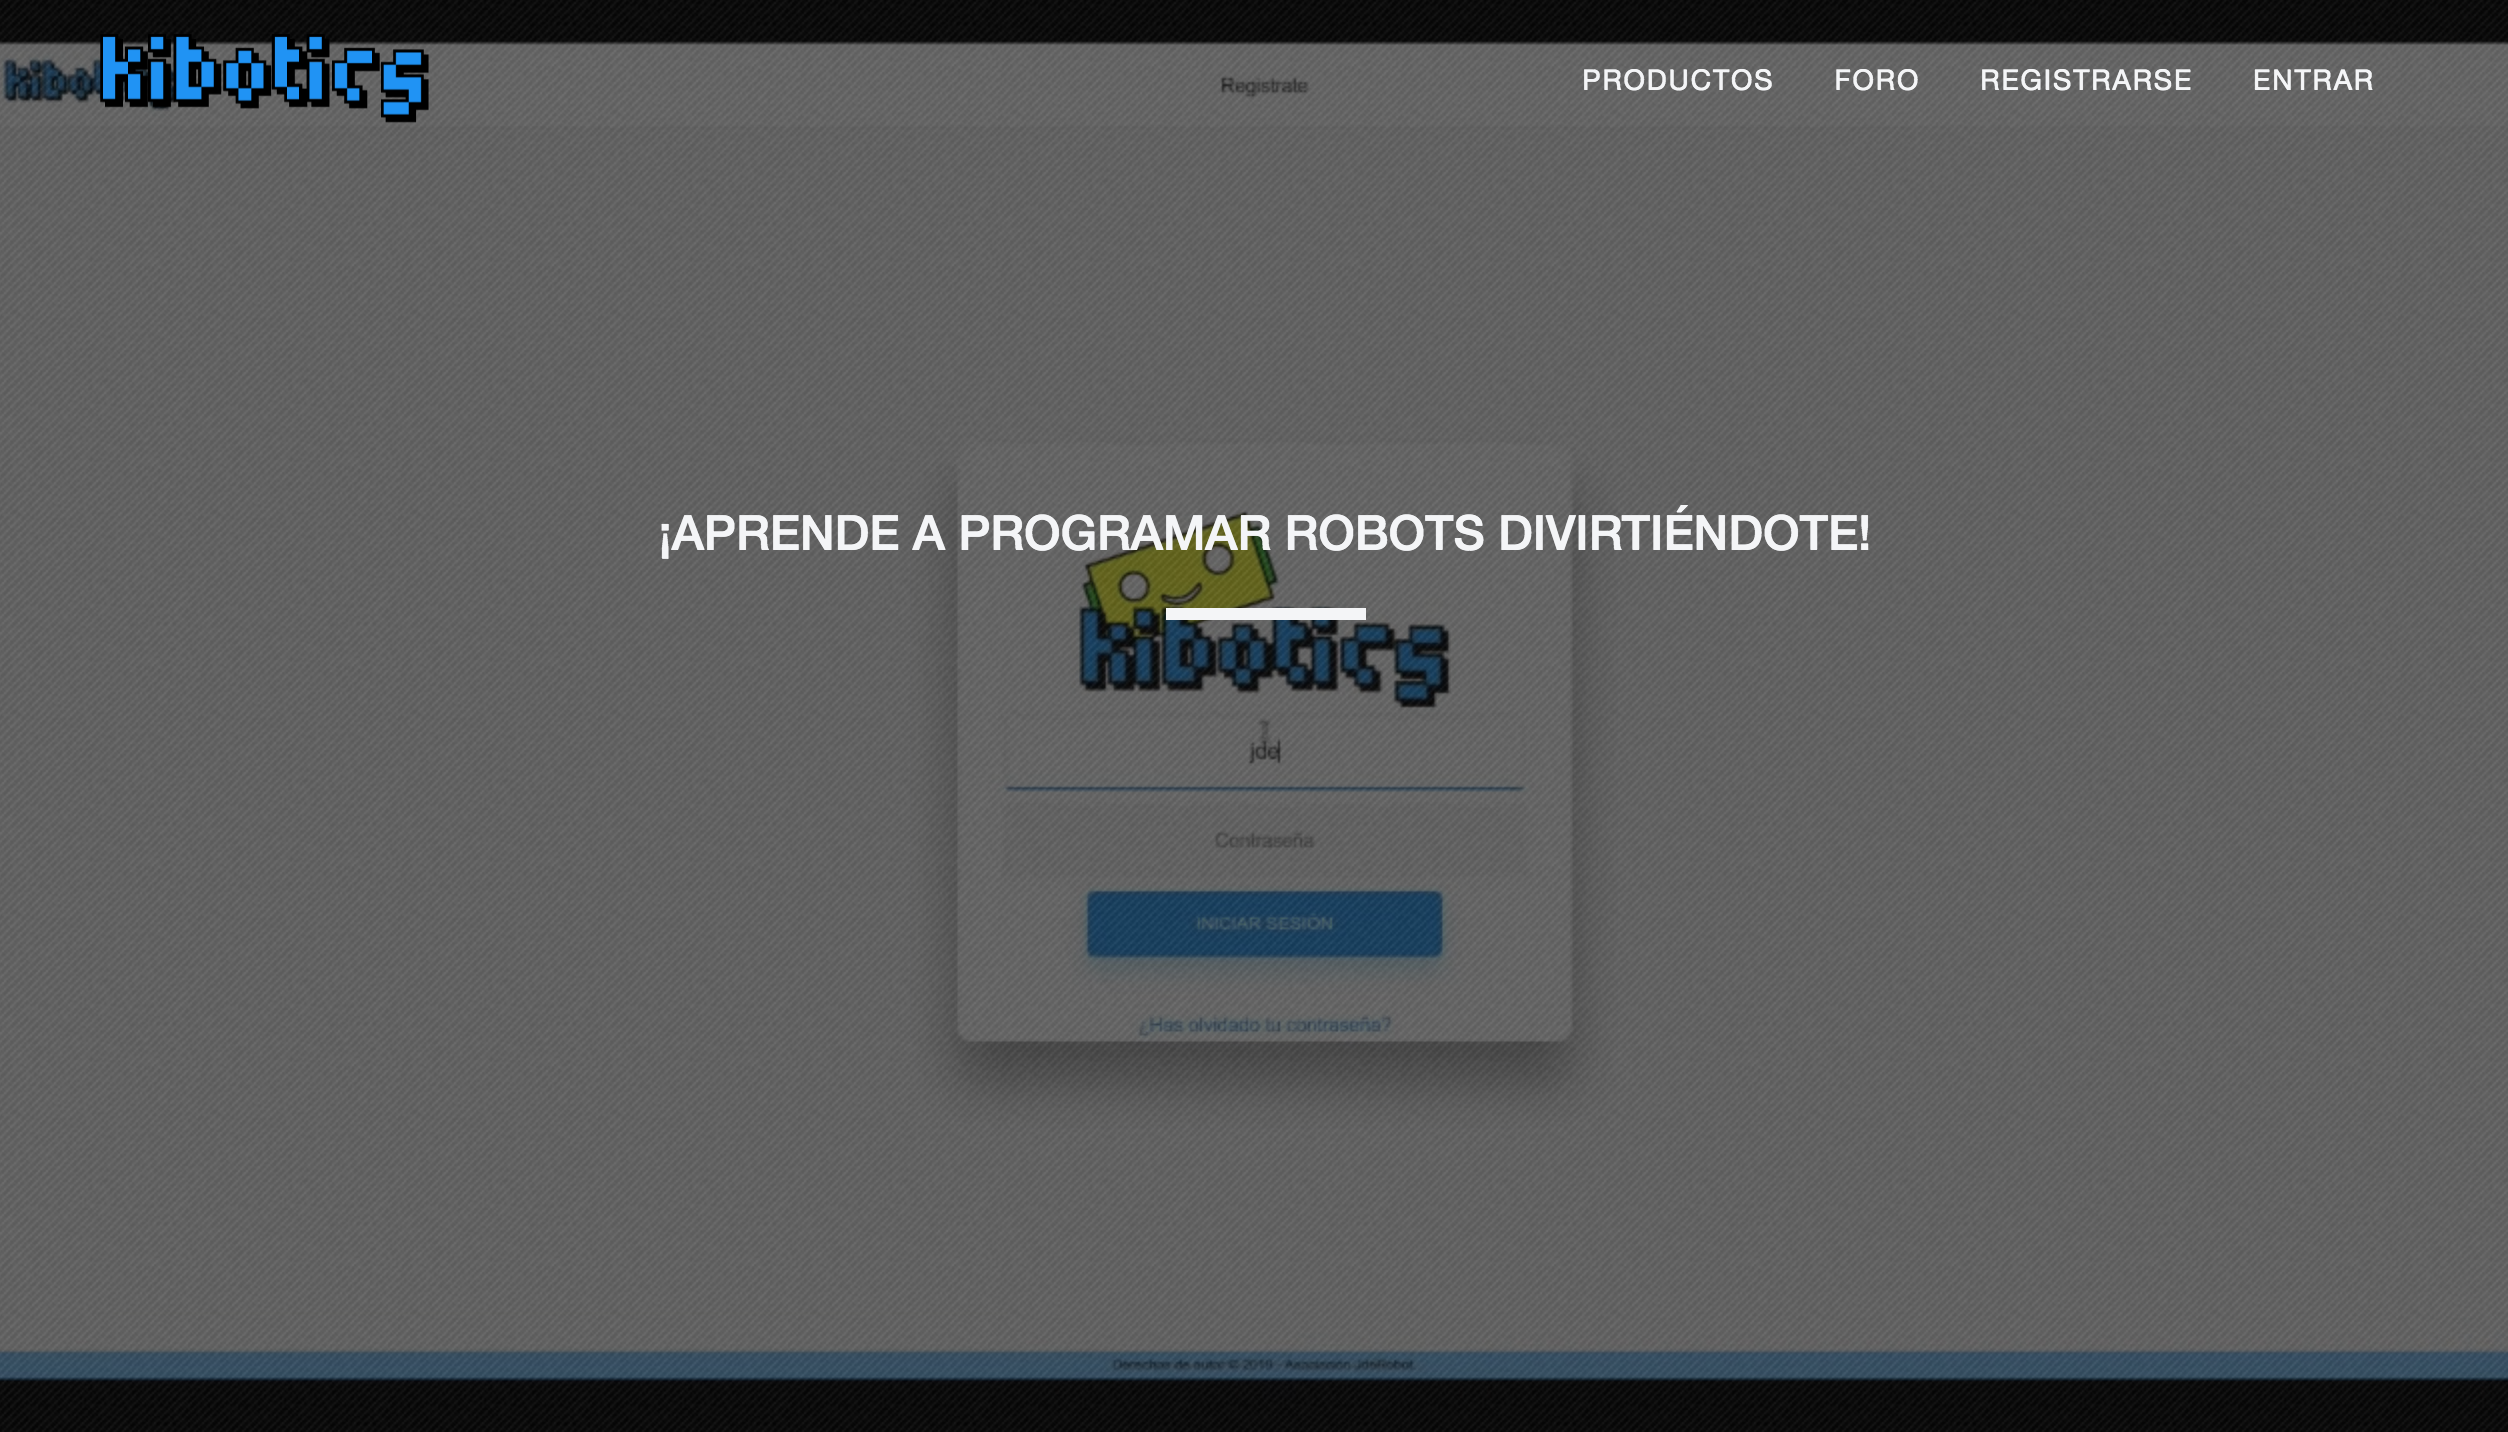
\includegraphics[width=0.9\textwidth, height=0.6\textwidth]{chapters/images/kiboticsorg.png}
    \caption{kibotics.org}
    \label{fig:f1}
  \end{subfigure}
  \hfill
  \begin{subfigure}[b]{0.5\textwidth}
  \centering
    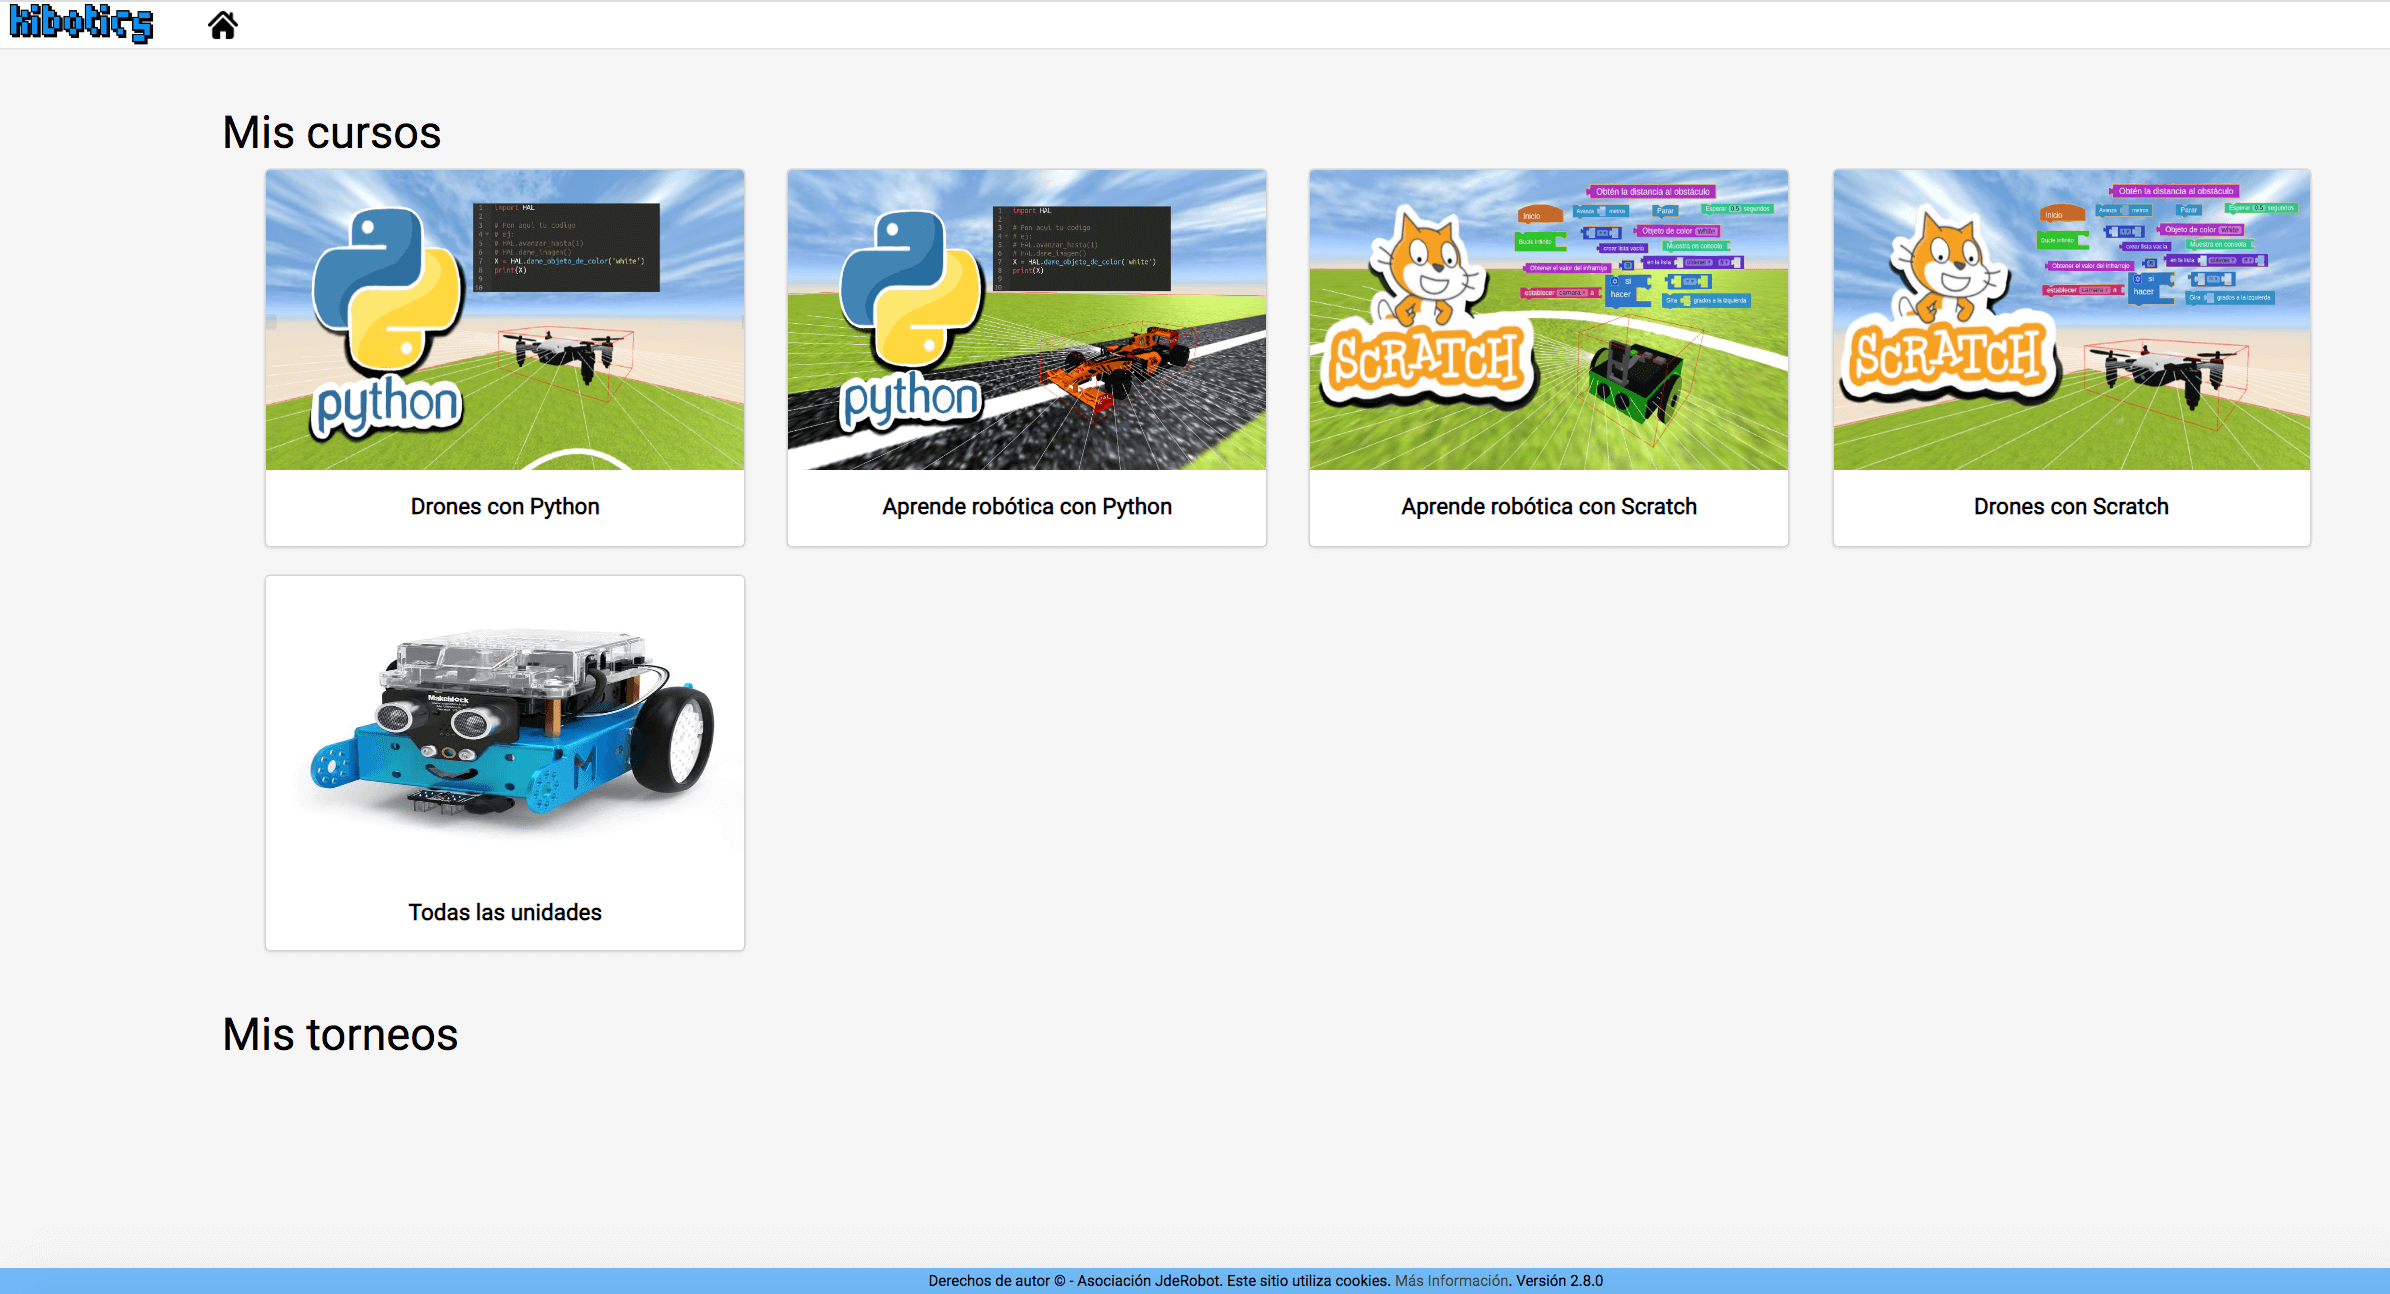
\includegraphics[width=0.9\textwidth, height=0.6\textwidth]{chapters/images/kibotics.png}
    \caption{Cursos disponibles en Kibotics.}
    \label{fig:f2}
  \end{subfigure}
  \caption{Plataforma Kibotics.}
\end{figure}
 
\subsection{Importancia de los juegos y multimedia en el aprendizaje} 
El planteamiento actual del sistema educativo tiene carencias y la innovación en la educación cobra cada vez más importancia. Es por ello que los docentes buscan actividades enfocadas en evitar la recurrente pasividad de los alumnos\cite{multimedia}.

Según el cono del aprendizaje de Edgar Dale y otros estudios concluyen que aprendemos un 10\% de lo que leemos, 20\% de lo que escuchamos, 75\% de lo que vemos y oimos y 
90\% de lo que hacemos \cite{videoeducativo}\cite{aprendizaje}. Estos porcentajes indican que, por lo tanto, la introducción del vídeo y los juegos interactivos en la clase puede producir modificaciones primordiales en el ámbito educativo.

La multimedia es un valioso recurso en la enseñanza por su naturaleza interactiva. Estos  materiales  deben ser adecuados y facilitar el aprendizaje. Para eso deben ser de fácil instalación y uso, versátiles, mostrar información de calidad e interactivos para motivar a los alumnos. Cada material se ajusta a los usuarios para que trabajen a su ritmo \cite{importanciamultimedia}.
\\
Las nuevas tecnologías están cada vez más interiorizadas en las aulas gracias al uso de pantallas, proyectores y ordenadores. La pandemia vivida en este último año ha impulsado el uso de aplicaciones web para dar clase como las plataformas de videoconferencia. Muchos profesores han optado por estas potentes plataformas, otros han grabado y compartido sus propios vídeos, donde los estudiantes pueden pararlos y verlos las veces necesarias para interiorizar mejor los conocimientos.
\\
En los últimos años se están incorporando juegos en las aulas como la apliación Kahoot! \cite{kahoot} en la que hacen juegos de encuestas, además se ha fomentado aprendizaje a través de vídeos y diapositivas más animadas, foros, así como el uso de plataformas educativas e interactivas como Moodle.
\\

 El término \textit{``Gamificación''} o ludificación se emplea para referirse al aprendizaje a través de juegos en el entorno educativo y profesional. Los juegos se utilizan para fomentar el aprendizaje de programación, mejorando los conocimientos y habilidades de los alumnos de una forma más dinámica y divertida. La Gamificación facilita la interiorización de los conocimientos, generando una respuesta positiva al usuario por cumplir con un objetivo.
 \\
 Enseñar a los más jóvenes cómo funcionan las últimas tecnologías y además les parezca entretenido e interesante es lo que nos ha motivado a realizar este trabajo.
 
 
\subsection{Campeonatos de robótica educativa existentes}

El aprendizaje de la robótica educativa ha ido más allá. Actualmente existen competiciones a nivel nacional e internacional que utilizan juegos y ejercicios competitivos \cite{competiciones}. Estas son algunas de ellas:
\begin{itemize}
    \item RoboCup Junior \footnote{https://junior.robocup.org/}: es una iniciativa educativa orientada a proyectos que patrocina eventos robóticos locales, regionales e internacionales para jóvenes estudiantes. Destaca la Liga de Rescate, Liga de Futbol (Figura 1.17(b)) y Liga ONSTAGE \cite{robocup}.
 
    \item Eurobot Junior\footnote{http://www.eurobot.es/}: es una competición europea de robots para estudiantes de primaria, secundaria o clubs de robótica. El grupo de jóvenes debe diseñar, construir y programar un robot telecontrolado por cable. Además pueden tener un robot secundario autónomo\cite{eurobot}.
    
    \item First Lego league \footnote{https://www.firstlegoleague.es/}: es un programa internacional  para jóvenes de 4 a 16 años a través de la resolución de problemas reales. Se adapta a cada edad con sus cursos Discover, Explore y Challenge\cite{firstlego}.
    
    \item Torneo Nacional VEX Robotics IQ\footnote{https://vexspain.com/}: destinado a equipos de 4 a 8 miembros de secundaria junto un adulto. Ofrecen distintos retos y torneos con premios\cite{vex}.
    
    \item RoboCampeones \footnote{http://robocampeones.org/}: Creado en el RoboticsLabURJC de la Universidad Rey Juan Carlos. Los alumnos de instituto compiten en pruebas como sumo con robots LEGO y Arduino. Se celebra en Fuenlabrada y en los últimos años contó con más de 2000 participantes (Figura 1.17(a)) \cite{robocampeones}.
    \\
    \\
    
    \begin{figure}[H]
  \begin{subfigure}[b]{0.5\textwidth}
  \centering
    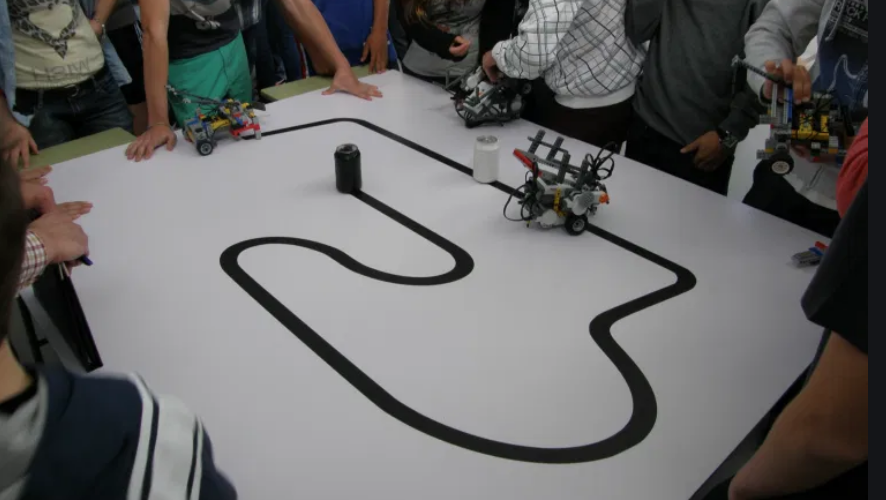
\includegraphics[width=0.95\textwidth, height=0.7\textwidth]{chapters/images/robocam.png}
    \caption{Juego Pañuelo Robocampeones}
    \label{fig:f1}
  \end{subfigure}
  \hfill
  \begin{subfigure}[b]{0.5\textwidth}
  \centering
    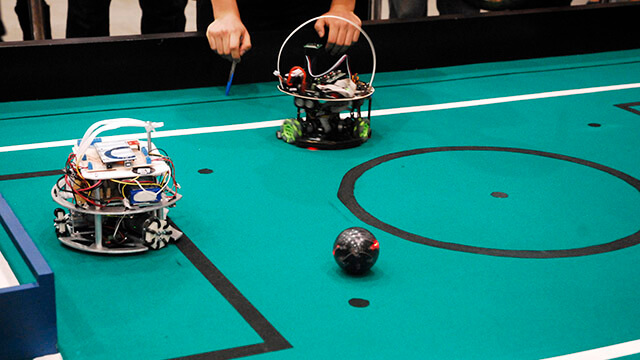
\includegraphics[width=0.95\textwidth, height=0.7\textwidth]{chapters/images/robocup.jpeg}
    \caption{Fútbol en RoboCup Junior.}
    \label{fig:f2}
  \end{subfigure}
  \caption{Campeonatos de robótica.}
\end{figure}
\end{itemize}

\newpage
\section{Estructura del documento}

La estructura de este trabajo fin de grado está compuesta por los siguientes capítulos:

\begin{itemize}
    \item \textit{Capítulo 1 Introducción}: una breve introducción a la robótica y tecnologías web para ponernos en contexto y presentar el tema principal del trabajo.
    \item \textit{Capítulo 2 Objetivos y Metodología}: Se fijan los objetivos concretos y se explica la metodología y plan de trabajo seguidos a lo largo de este proyecto.
    \item \textit{Capítulo 3 Infraestuctura utilizada}: se describen lenguajes, tecnologías y herramientas empleadas en este trabajo.
\end{itemize}

Para una mejor exposición del trabajo que se ha realizado, el desarrollo se ha dividido en 3 capítulos, de esta forma nos centraremos en el enunciado, la infraestructura y solución de referencia de cada ejercicio:
    
\begin{itemize}
   \item \textit{Capítulo 4 Ejercicio Teleoperador Acústico y Banda Sonora}
    \item \textit{Capítulo 5 Ejercicio Aspiradora robótica atrapa confeti}
    
    \item \textit{Capítulo 6 Ejercicio Juego del pañuelo}

    
    \item \textit{Capítulo 7 Conclusiones y trabajos futuros}: Conclusiones del trabajo y futuros proyectos posibles a partir de este.
  \end{itemize}
